\clearpage
\section{Energy regressions for photons and electrons in the 2016 dataset}
\label{app:regression}

\newcommand{\Eraw}{\ensuremath{E_\text{raw}}\xspace}
\newcommand{\Etrue}{\ensuremath{E_\text{true}}\xspace}
\newcommand{\Ecorr}{\ensuremath{E_\text{corr}}\xspace}

The energy of reconstructed photons and electrons is measured by translating the detected amount of light in the scintillating lead-tungstate crystals into energy measurements per crystal, and summing the energy of crystals within a specified region called the \textit{supercluster}.
% 
This summed energy measurement yields what is called the \textit{raw energy} $\Eraw$; it is the baseline for further corrections, which are designed to approximate the \textit{true energy} $\Etrue$ as closely as possible.
% 
These corrections are required mostly to solve the lack of containment of the particle's energy deposit within CMS ECAL.
% 
For example, gaps in between the crystals and modules may cause some deposited energy not to be reconstructed, a problem referred to as limited \textit{local containment}.
% 
In addition, there is a non-negligible amount of material in between the interaction point and ECAL, leading to photon conversions and bremsstrahlung for electrons.
% 
The radiated particles from these effects are typically bent along the $\phi$ direction due to the strong magnetic field, and may on occasion fail to be included in the determination of the supercluster~\cite{Chatrchyan:2013dga}.
% 
This problem is referred to as limited \textit{global containment}.
% 
The procedure of obtaining an estimate of $\Etrue$ from $\Eraw$ is called the \textit{energy regression}.


The regression is carried out via a \textit{semiparametric boosted decision tree} (BDT), which is a boosted decision tree that in its leafs contains a parametrization of the target.
% 
This type of multivariate analysis is called `semiparametric' as the product is parametric, but the decision tree itself is determined the same way as a regular BDT, independent of an a priori parametrization.
% 
The parametric form chosen in the leafs is a so-called \textit{double-sided crystal ball function} (DCSB) function, with the following algebraic form~\cite{Aad:2015oqa}:
% 
\begin{linenomath*}
\begin{equation}
\label{eq:dscb}
\text{DCSB}(x) = \left\{
    \begin{array}{ll}
    \exp{-\alpha_L^2/2}
        \left( 1-\frac{\abs{\alpha_L}}{n_L} \left(\abs{\alpha_L}+t\right) \right)^{-n_L}
        & \text{if} \quad t \leq -\alpha_L, \\
    % 
    \exp{-t^2/2} & \text{if} \quad -\alpha_L < t < \alpha_R, \\
    % 
    \exp{-\alpha_R^2/2}
        \left( 1-\frac{\abs{\alpha_R}}{n_R} \left(\abs{\alpha_R}+t\right) \right)^{-n_R}
        & \text{if} \quad t \geq \alpha_R, \\
    \end{array}
    \right.
\end{equation}
\end{linenomath*}
% 
where $t = \frac{x-\mu}{\sigma}$, and $\mu$, $\sigma$, $\alpha_{L/R}$ and $n_{L/R}$ are parameters of the DSCB; importantly, $\mu$ and $\sigma$ are the mean and standard deviation of the Gaussian core of the function.
% 
For the regression performed here, $\alpha_L$ has been fixed to 2, and $\alpha_R$ to 1; these constant values seem to work well throughout the energy regime, and fixing them allows the BDT to learn the more important parameters of the Gaussian core with greater success.
% 
The regression takes as input a number of variables from ECAL, such as the raw energy, the location of the supercluster in the detector, the width and height of the supercluster in terms of $\eta$ and $\phi$, and the ratio of the total energy measured in HCAL over the total energy measured in ECAL.
% 
The most important variables, however, pertain to the \textit{shower shape} of the electron or photon; notable examples include \textit{R9}, defined as the ratio of the summed energy of the $3\times3$-cluster around the electron or photon over the energy of the supercluster, and ratios of various crystal arrays over the summed energy of the $5\times5$-cluster around the electron or photon.
% 
In the case of electrons, a second set of variables is available from the tracker; these are mostly important for low-energy electrons.
% 
The regression is performed separately for the barrel and endcap regions, and as such the input variables also differ slightly; for example, in the endcap regions the preshower energy measurement is included as an input, and rather than $\eta$ and $\phi$, the locations of the superclusters are given in planar coordinates.


For low-energy electrons, the most prominent variables for the energy correction are those from the tracker.
% 
While an obvious fact from physics considerations, in a BDT these type of trivialities must be learned through the analysis of large amounts of data.
% 
In order to speed up the training, increase chances of convergence, and to improve the final result, it is typically preferable to design the training with these given facts in mind.
% 
The energy regression for electrons is determined by first training a BDT using only ECAL variables.
%
As a target function, which is to be brought as closely to 1 as possible via multiplication with the to-be-determined correction with minimal standard deviation per leaf, it uses
% 
\begin{linenomath*}
\begin{equation}
\text{target}_1 = \frac{\Etrue}{\Eraw}
\,.
\end{equation}
\end{linenomath*}
% 
The corrected energy $\Ecorr$ that is yielded by this BDT is already a good estimate of $\Etrue$, and for energies ${>}100\GeV$ it is basically the final estimate.
% 
Subsequently, a second BDT is trained, this time including the tracker variables, with the target defined as
% 
\begin{linenomath*}
\begin{equation}
\text{target}_2 = 
% 
\frac{\Etrue}{E_\text{estimate}} =
% 
\frac{\Etrue}{ w_\text{ECAL} \Ecorr + w_\text{tracker} \abs{p} }
\,,
\end{equation}
\end{linenomath*}
% 
where $\abs{p}$ is the absolute momentum determined from the tracker, and the weights are defined as
% 
\begin{linenomath*}
\begin{equation}
w_\text{ECAL} = \left( \frac{\sigma^2_{\abs{p}}}{\sigma^2_{\abs{p}} + \sigma^2_{\Ecorr}} \right)
\;,\quad
w_\text{tracker} = \left( \frac{\sigma^2_{\Ecorr}}{\sigma^2_{\abs{p}} + \sigma^2_{\Ecorr}} \right)
\,.
\end{equation}
\end{linenomath*}
% 
The denominator is essentially a weighted sum of the energy estimations from the tracker and from ECAL, where the weights are determined by the respective uncertainties.
% 
With this two-tiered approach, the regression has only to learn in the second stage to trust the tracker energy estimate more for low-energy electrons, and the ECAL estimate for high-energy electrons, greatly reducing the required training time and improving the chances for convergence.
% 
Histograms of the weights for increasing electron $\pt$ are shown in Fig.~\ref{fig:regressionweights}; for very low $\pt$, the tracker weight is typically larger, whereas for a larger $\pt$ the weight assigned to the corrected ECAL energy measurement is larger.


\begin{figure}[hbtp]
  \begin{center}
    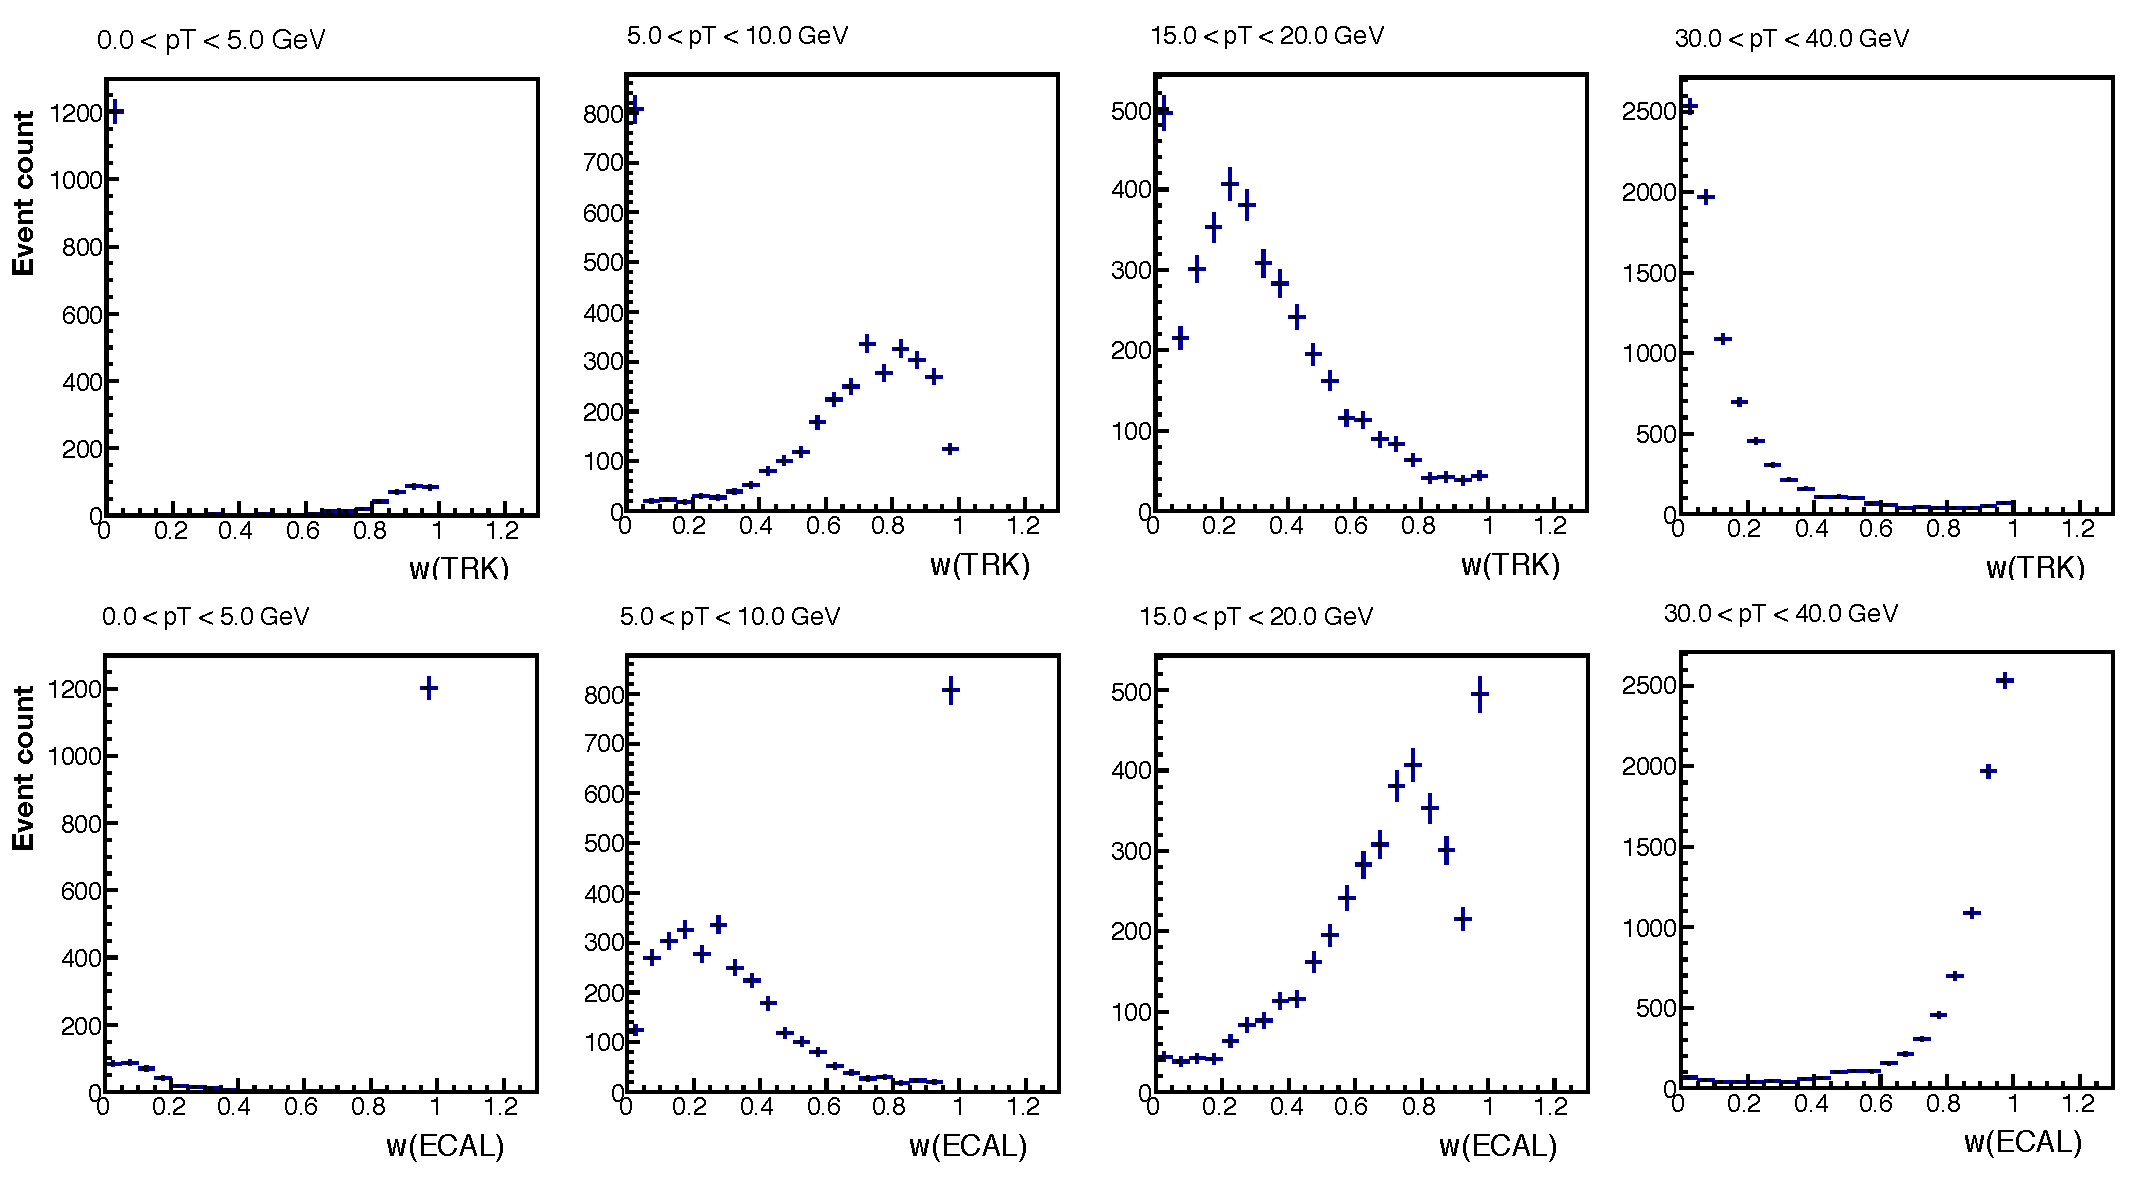
\includegraphics[width=0.99\linewidth]{img/regression/weightplot.pdf}
    \caption{
        Weights based on uncertainties in energy resolution for the tracker energy measurement (top row) and the ECAL energy measurement (bottom row), for increasing electron $\pt$.
        %
        For larger electron $\pt$, the weight assigned to the corrected ECAL energy measurement from the first BDT is larger, whereas for small electron $\pt$ the weight assigned to the energy estimate from the tracker is larger.
        % 
        For a particular subset of events, the tracker energy resolution is, by chance, very poor; this leads to a nearly full weight placed on the ECAL energy measurement in these cases, visible as a peak at 1.0 in the $w_\text{ECAL}$ histograms.
        }
    \label{fig:regressionweights}
  \end{center}
\end{figure}


With respect to previous versions of this regression (meant for data collected by the CMS detector before 2016), the results described here include variables pertaining to \textit{crystal saturation}, the effect that occurs when the deposited energy exceeds the maximum allowed value of the readout electronics.
% 
This effect occurs for energy deposits greater than approximately $2000\GeV$, and severely deteriorates the energy scale and resolution.
% 
The effect is illustrated in Fig.~\ref{fig:saturation}; it is clear that for high-energy electrons, $\Eraw$ underestimates $\Etrue$ by a wide margin.
% 
To mitigate this effect, the first stage of the regression takes the number of saturated crystals as an input variable.
% 
Interestingly, this single variable increases the performance of the regression drastically in the high energy regions, and adding more information pertaining to crystal saturation does not significantly improve the results.
% 
The corrected energy including the number of saturated crystals as a variable is shown in Fig.~\ref{fig:saturation_corrected}.
% 
Unlike the raw energy measurement, the corrected energy shows no drastic underestimation with respect to the true energy.


\begin{figure}[hbtp]
  \begin{center}
    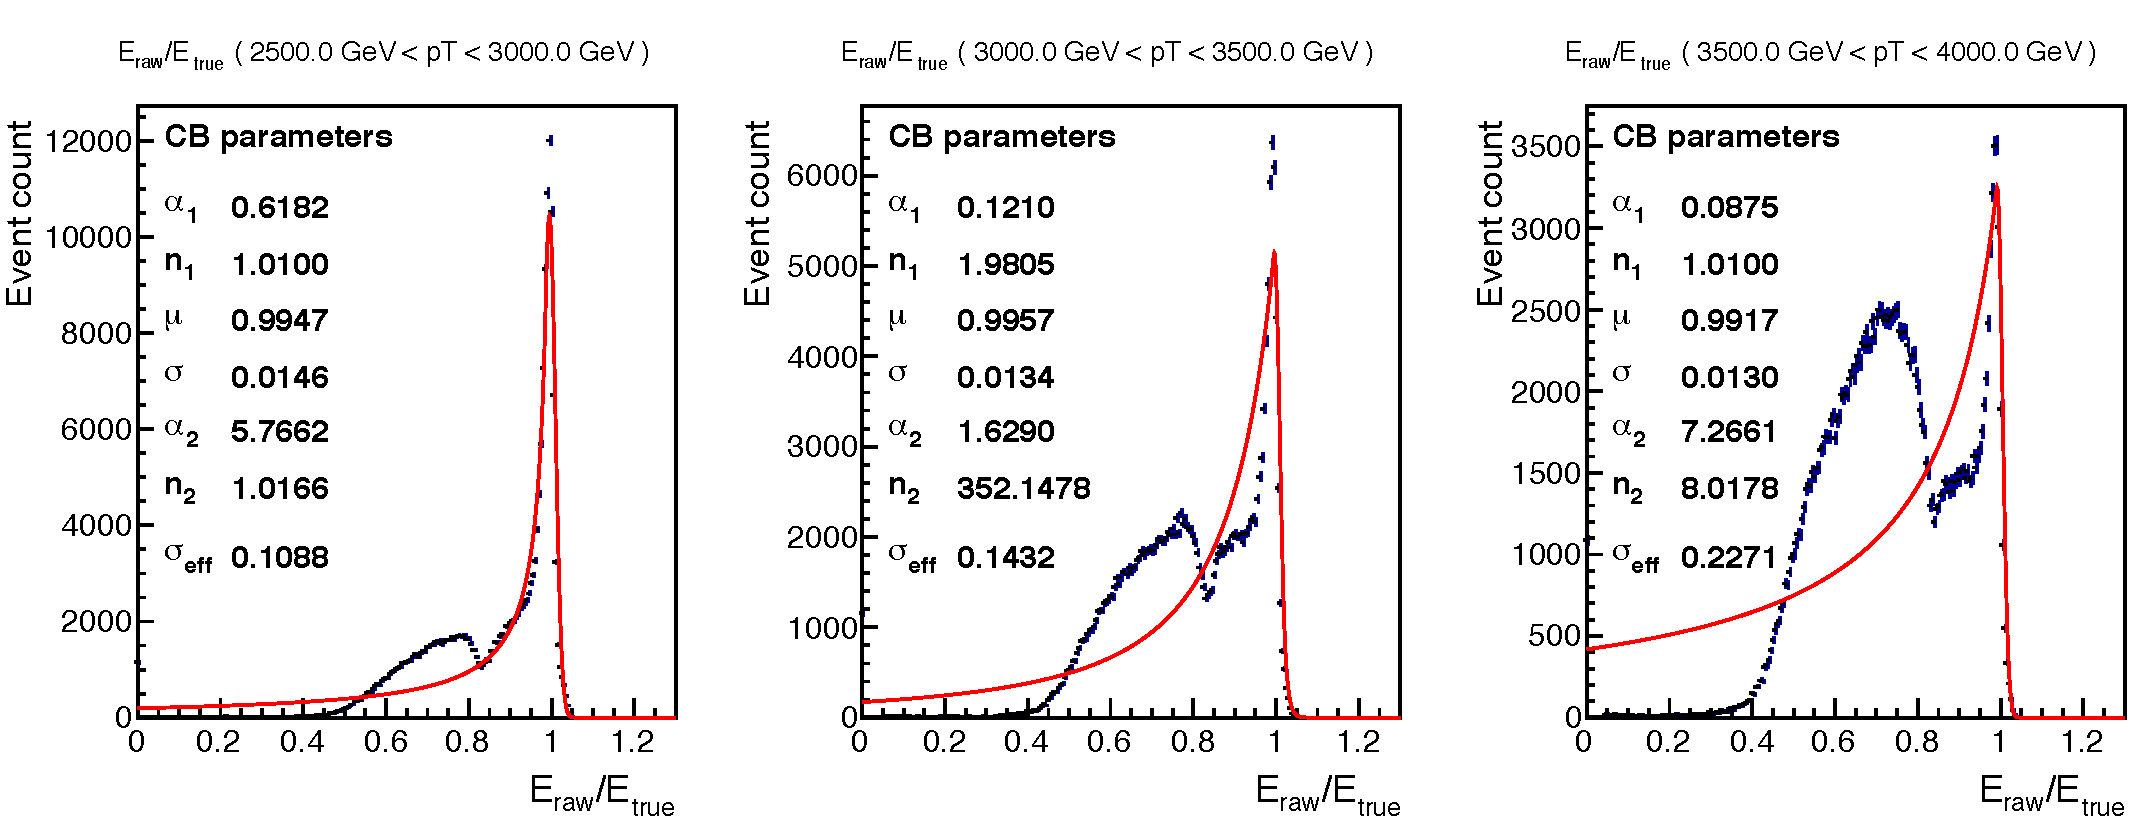
\includegraphics[width=0.99\linewidth]{img/regression/saturation.pdf}
    \caption{
        Example of crystal saturation for high-energy electrons.
        % 
        The red line is a DSCB fit to the histogram.
        % 
        The ratio of $\Eraw$ over $\Etrue$ is close to 1.0 when crystals are not saturated; in these cases the uncorrected energy measurement is not too far off from the true energy.
        % 
        However, for high-energy electrons more crystals saturate, and the raw energy strongly underestimates the true energy.
        }
    \label{fig:saturation}
  \end{center}
\end{figure}

\begin{figure}[hbtp]
  \begin{center}
    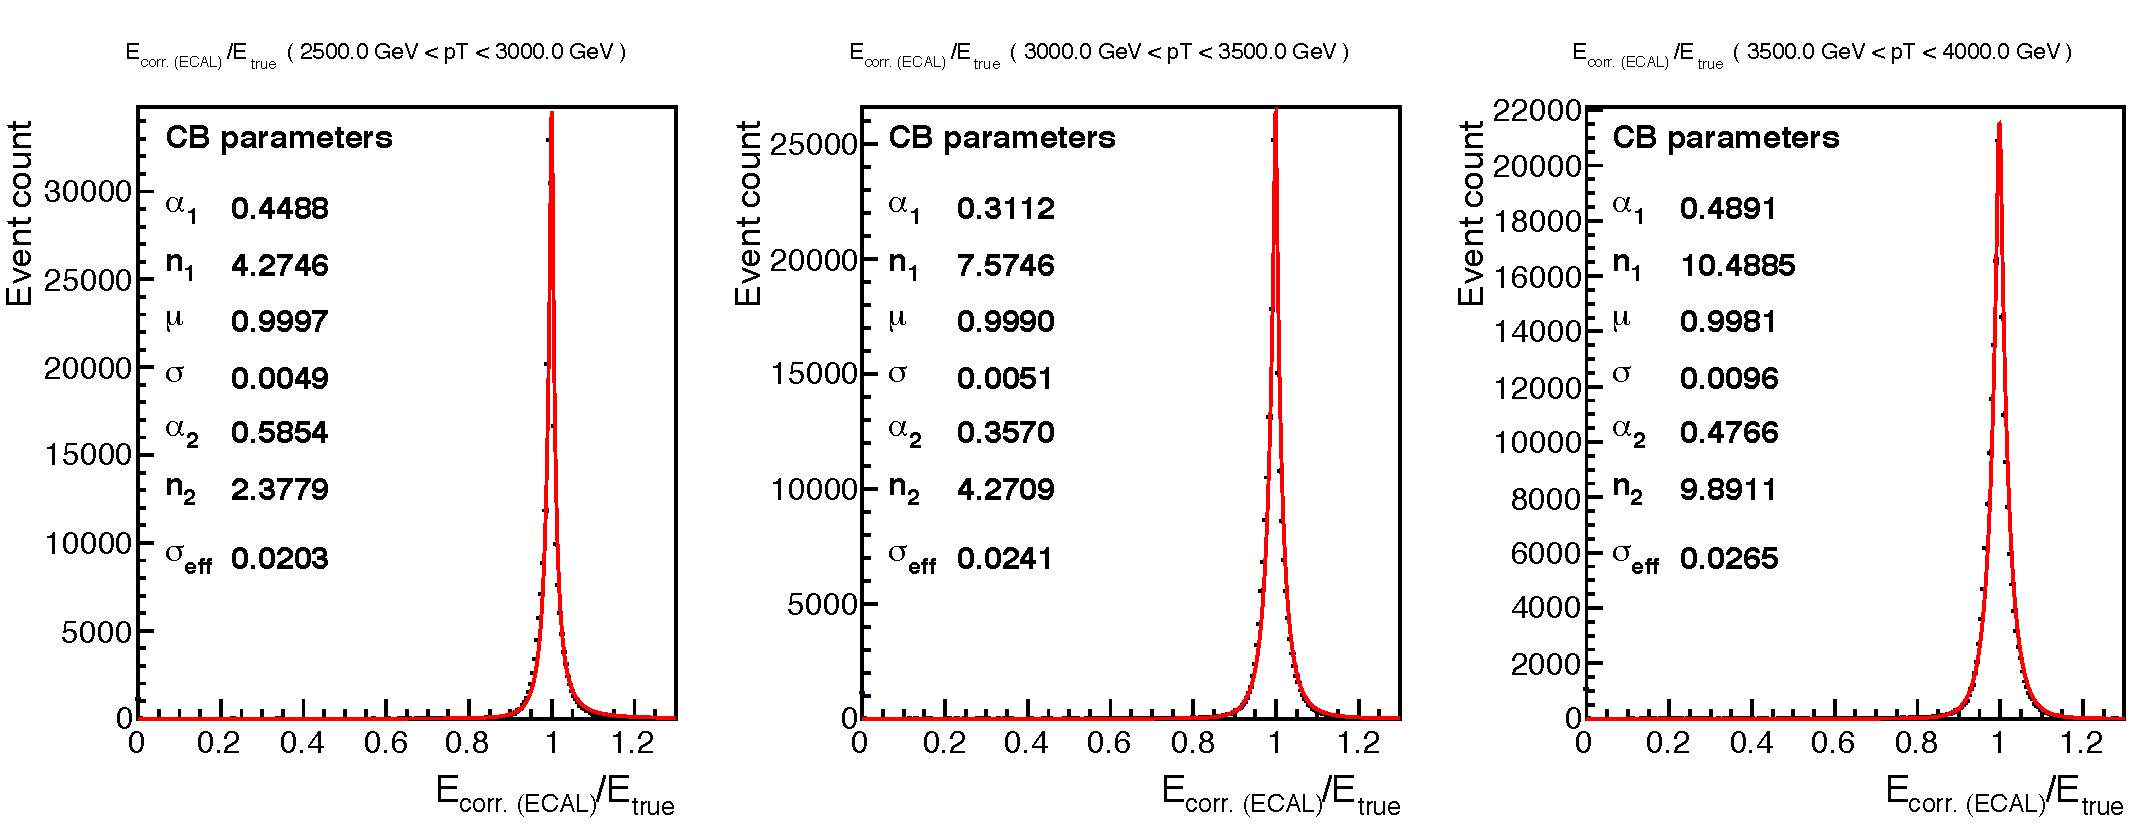
\includegraphics[width=0.99\linewidth]{img/regression/saturation_corrected.pdf}
    \caption{
        Corrected energy estimate for electrons, using only the first stage of the training (i.e.\ without any information from the inner tracker).
        % 
        The red line is a DSCB fit to the histogram.
        % 
        The corrected energy is a very good estimate of the true energy, despite the relatively large number of saturated crystals in this region of phase space.
        }
    \label{fig:saturation_corrected}
  \end{center}
\end{figure}


The scale, defined as the parameter $\mu$ of the DSCB in Equation~\ref{eq:dscb}, is plotted in Fig.~\ref{fig:pt100_scale} as a function of $\pt$ (up to 100\GeV) for electrons (left) and photons (right) for various stages of the regression, including the corrected energies under a previous version of the regression.
% 
The raw energy measurement is clearly a poor estimate of the true energy, not reaching percent-level precision for the lower part of the $\pt$ spectrum.
% 
The first stage (and final stage in the case of photons) of the regression brings the scale within per-mille level agreement with respect to the true energy, and provides an evident improvement with respect to the previous version of the regression.
% 
Around $50\GeV$, the scale using only ECAL variables in the case of electrons seems to deviate sharply from the trend; this deviation is merely a poor determination of the parameter $\mu$ from the histogram, and is of no concern for the actual performance of the regression.
% 
% Similar misdeterminations occur frequently in the results that follow, and will be pointed out where needed.


\begin{figure}[hbtp]
  \begin{center}
    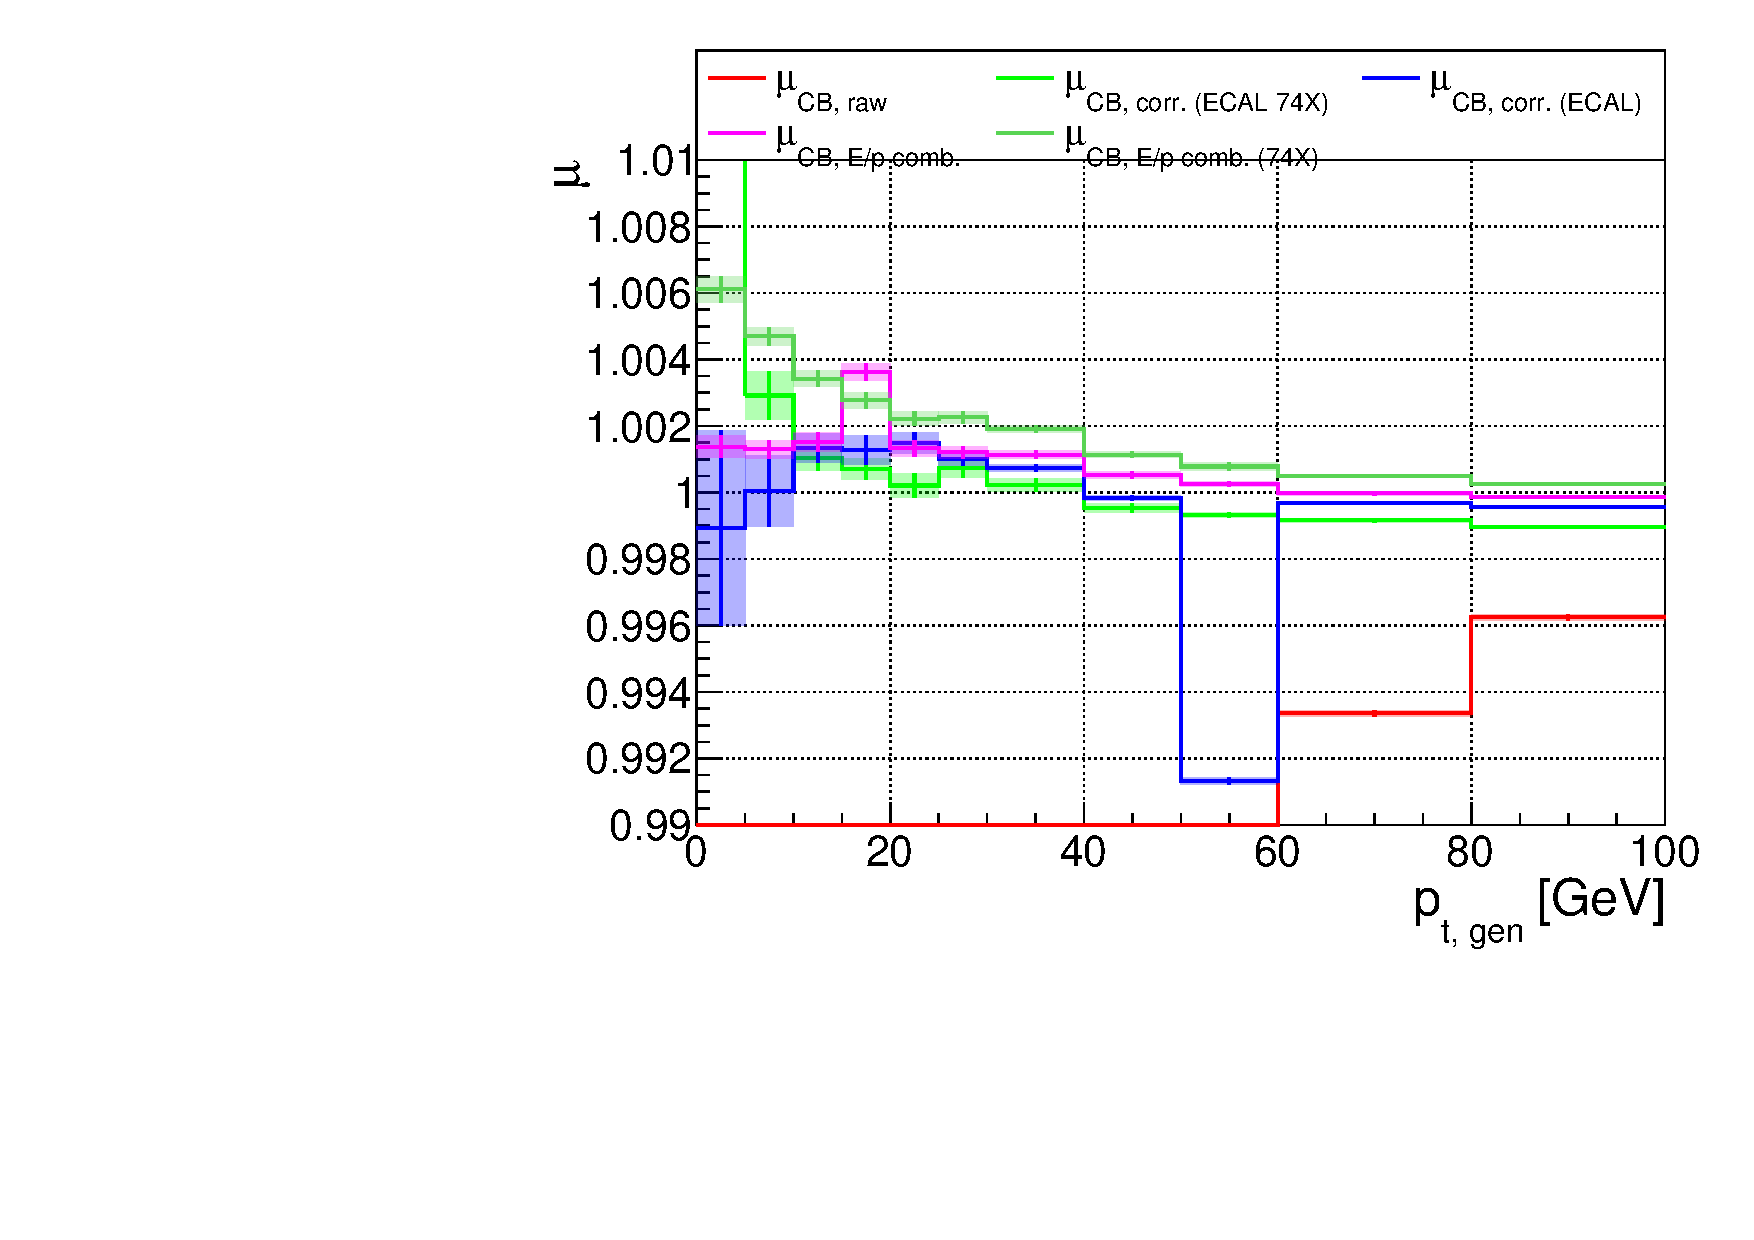
\includegraphics[width=\halflinewidth]{img/regression/pt100_scale_electrons.pdf}
    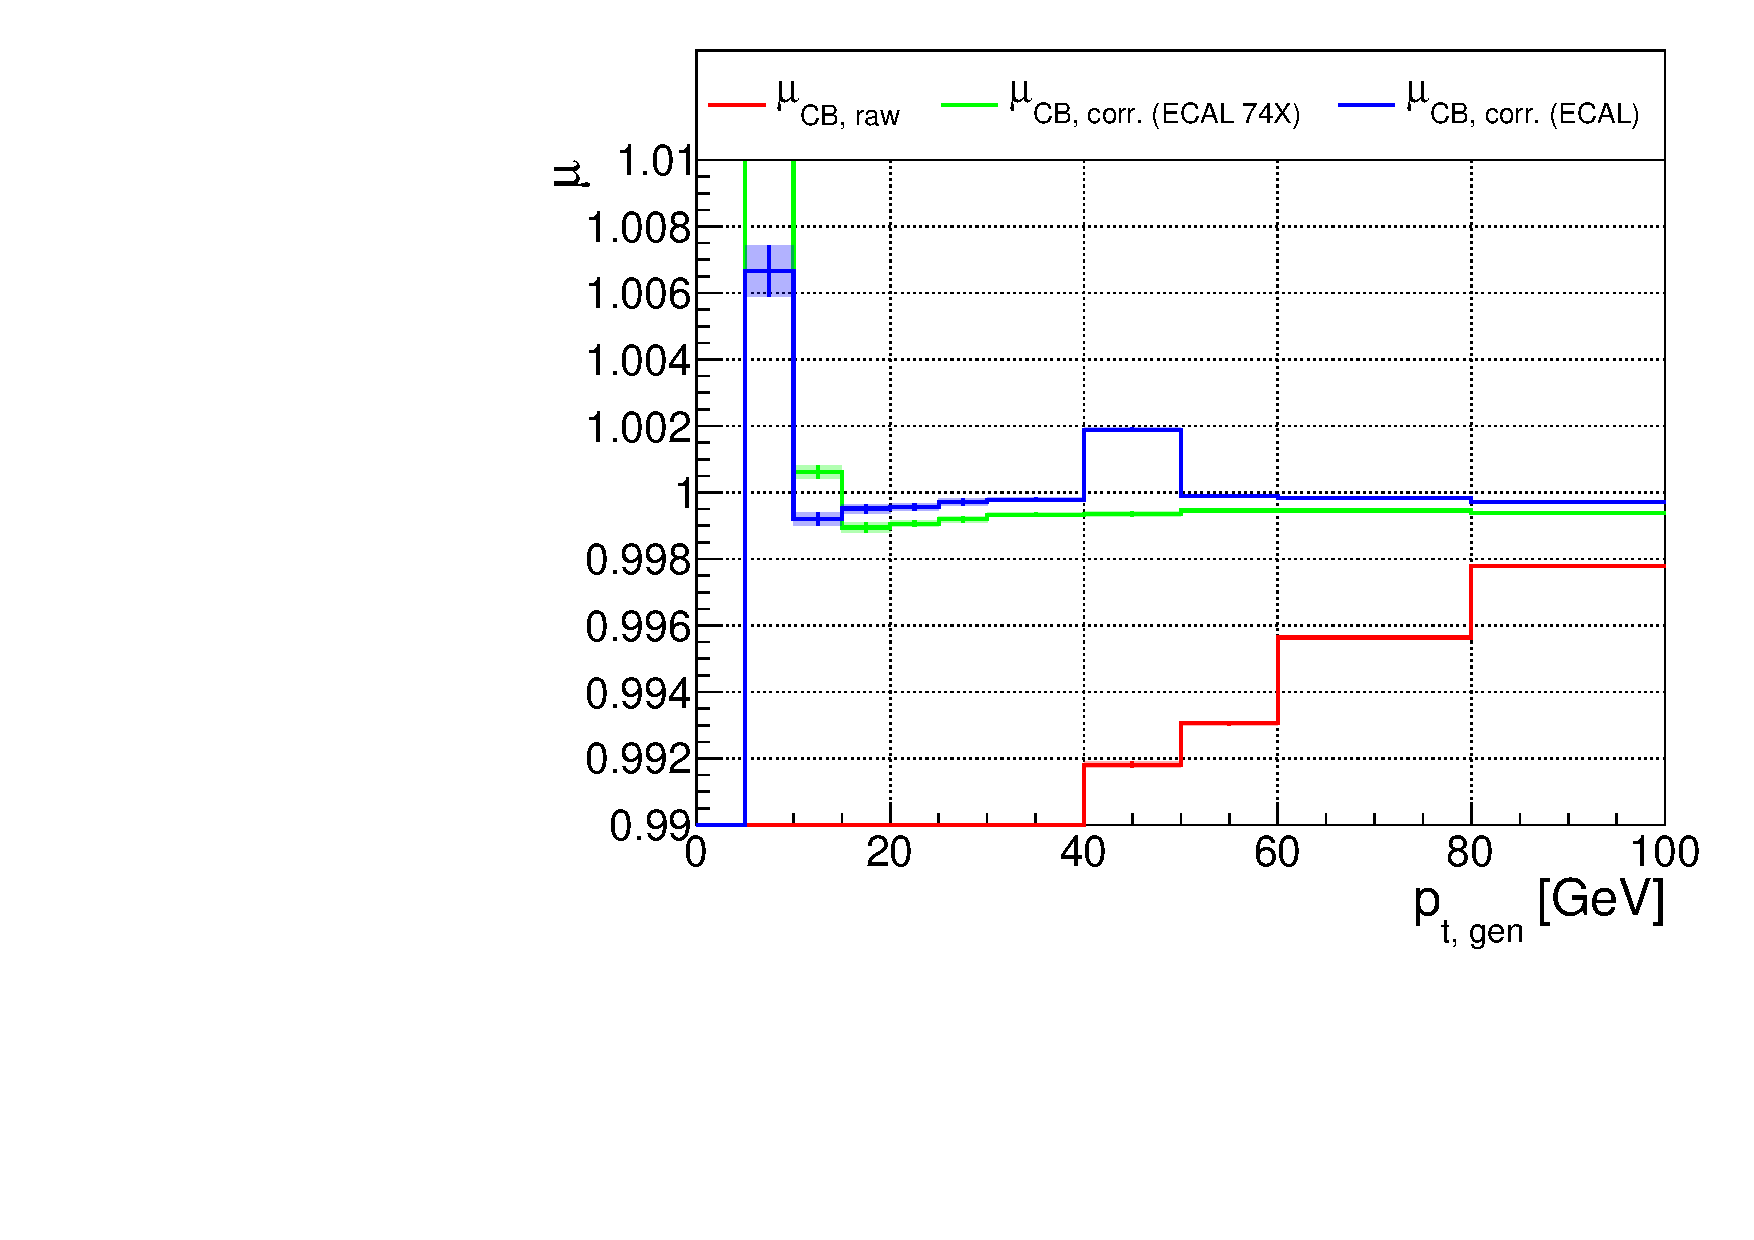
\includegraphics[width=\halflinewidth]{img/regression/pt100_scale_photons.pdf}
    \caption{
        The energy scale for electrons (left) and photons (right) as a function of $\pt$ for the raw energy (red), the corrected energy using only information from ECAL (blue), and the corrected energy using also variables from the input tracker in the second stage of the regression (pink).
        % 
        The corrected energies of the first and second stages are also given for a previous version of the regression, marked ``74X'', in light and dark green, respectively.
        }
    \label{fig:pt100_scale}
  \end{center}
\end{figure}


Figure~\ref{fig:effsigma} shows $\sigma_\text{eff}$, defined as the half width of the 1-standard-deviation interval around the geometrical mean of the histogram and meant to indicate the quality of the energy resolution, as a function of $\pt$.
% 
The enhanced resolution of the final stage of the regression with respect to the raw energy and the first stage of the regression is clearly visible in the electron $\pt$ spectrum, starting at a resolution of about 5\% and steadily improving to about 1\%.
% 
With respect to the previous version of the regression, the resolution does not improve significantly, unlike the correctness of the scale.
% 
Up until around 1500\GeV the resolution stays stable at around 1\% for both electrons and photons, and deteriorates around 1500\GeV, where saturation starts affecting the resolution.
% 
Whereas the raw energy and the previous energy regression deviate strongly, the newly obtained regression barely loses percent-level precision up until 2500\GeV.
% 
Also the correctness of the scale is improved with respect to the raw energy and the previous energy regression, as is shown in Fig.~\ref{fig:pt2500_scale}; the scale of the regression is within per mille level of the true energy.


\begin{figure}[hbtp]
  \begin{center}
    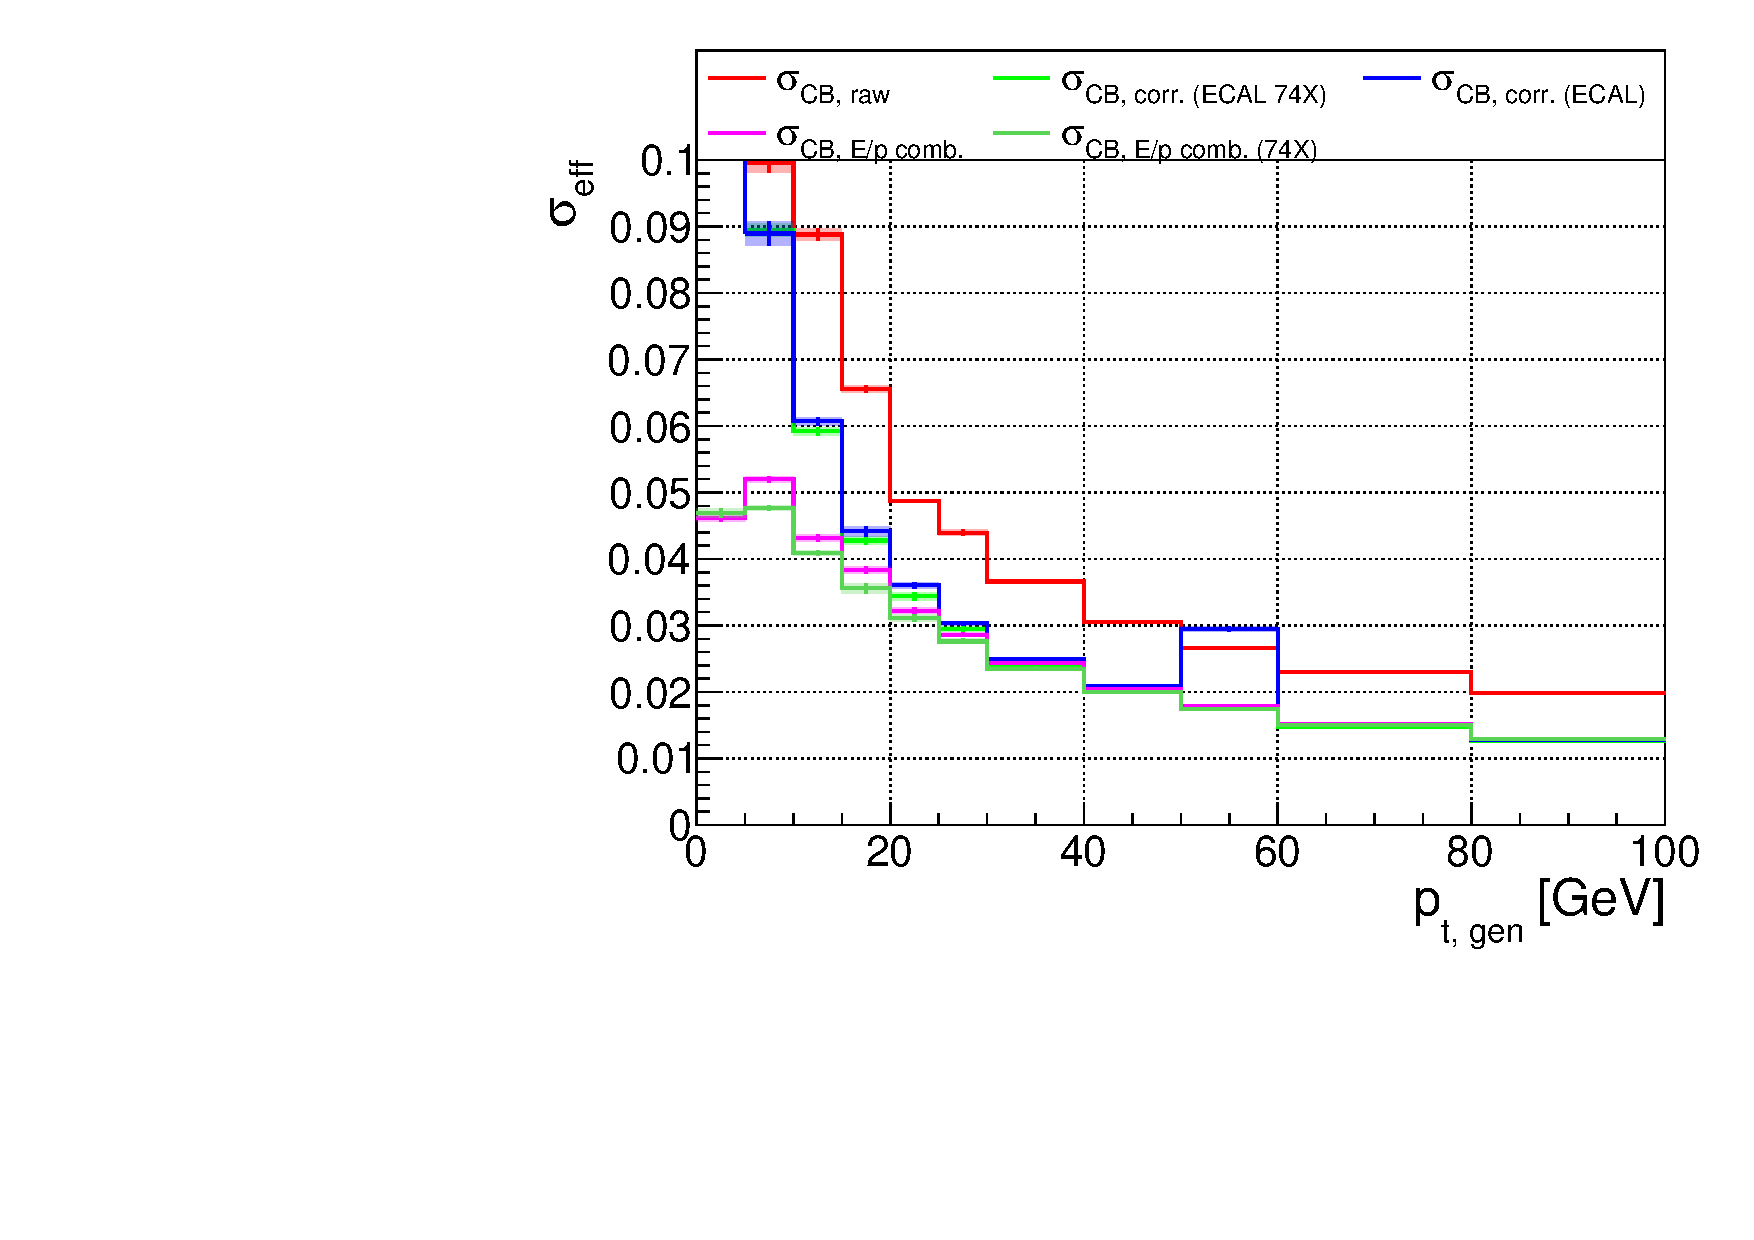
\includegraphics[width=\halflinewidth]{img/regression/pt100_effsigma_electrons.pdf}
    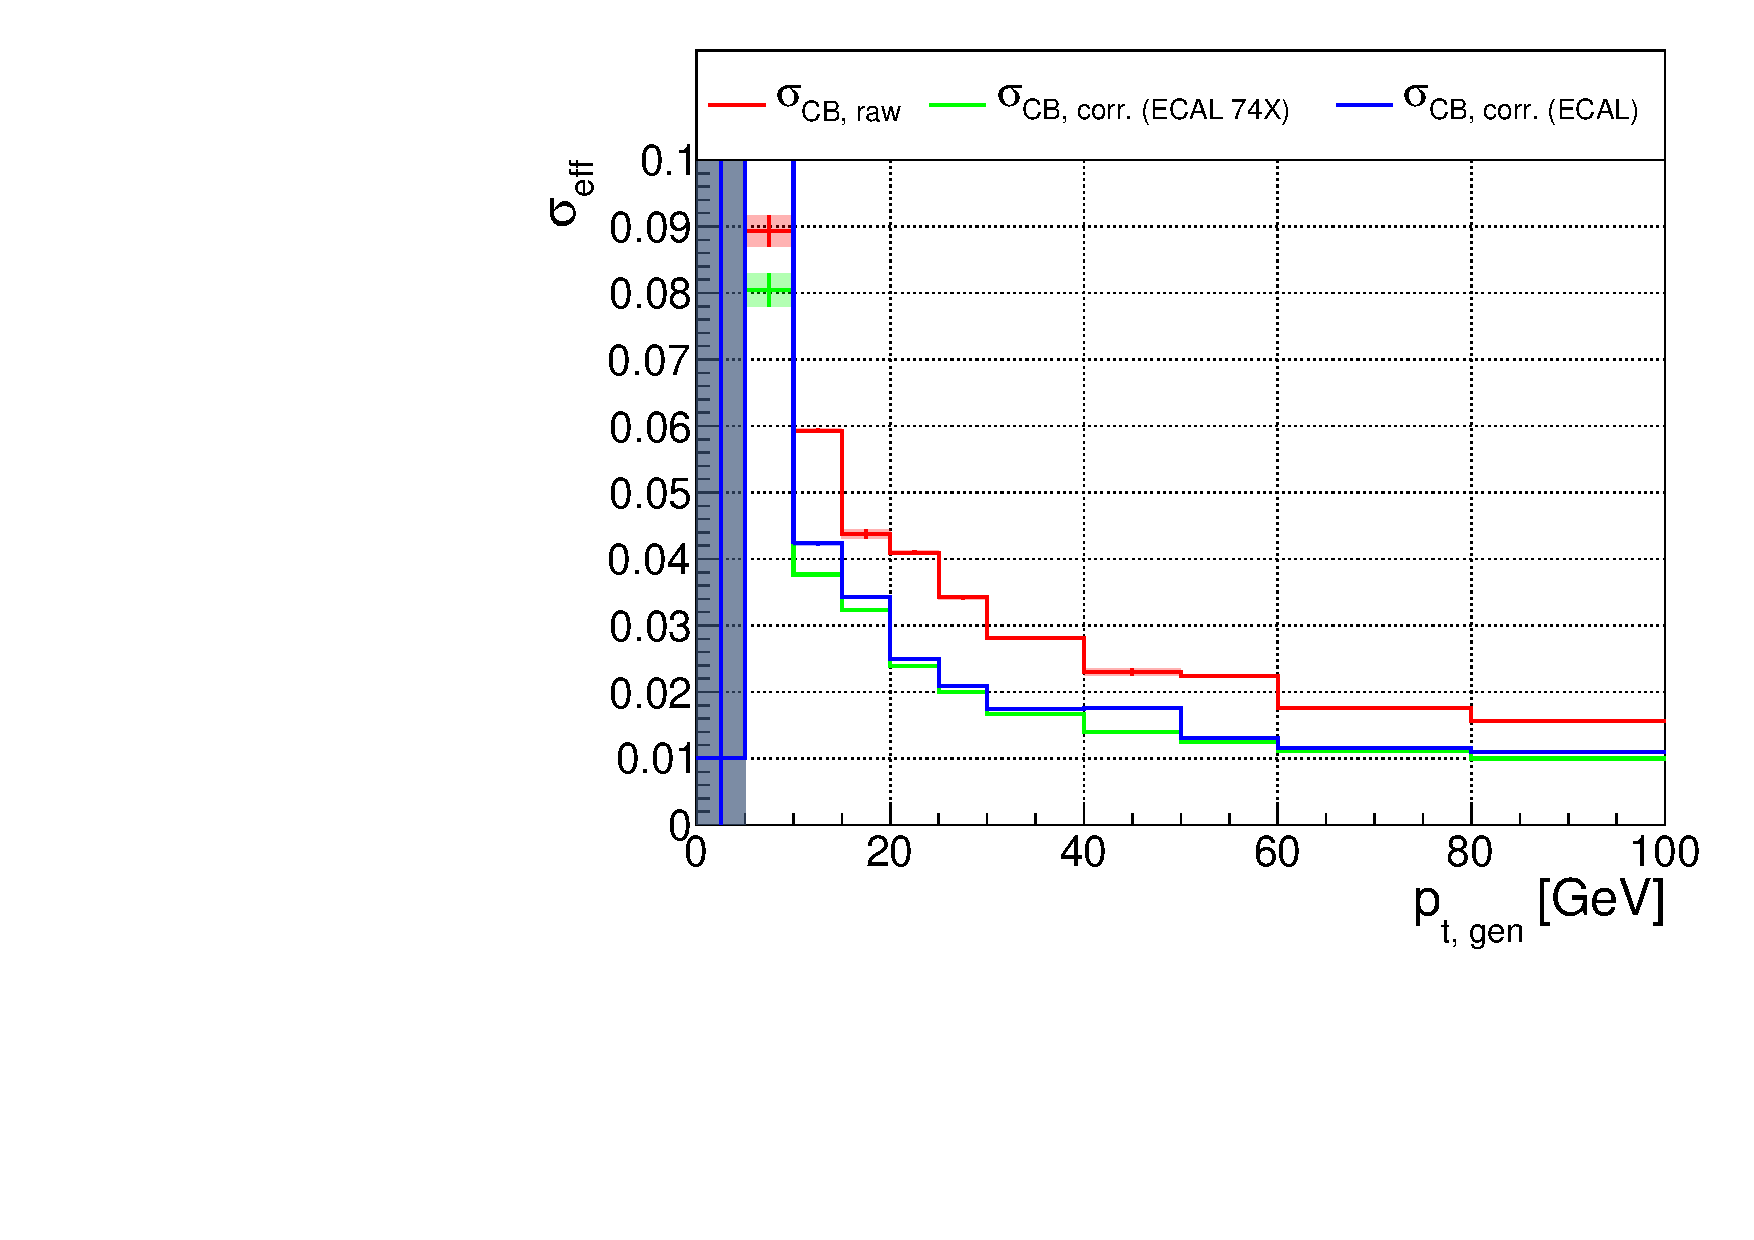
\includegraphics[width=\halflinewidth]{img/regression/pt100_effsigma_photons.pdf}
    \\
    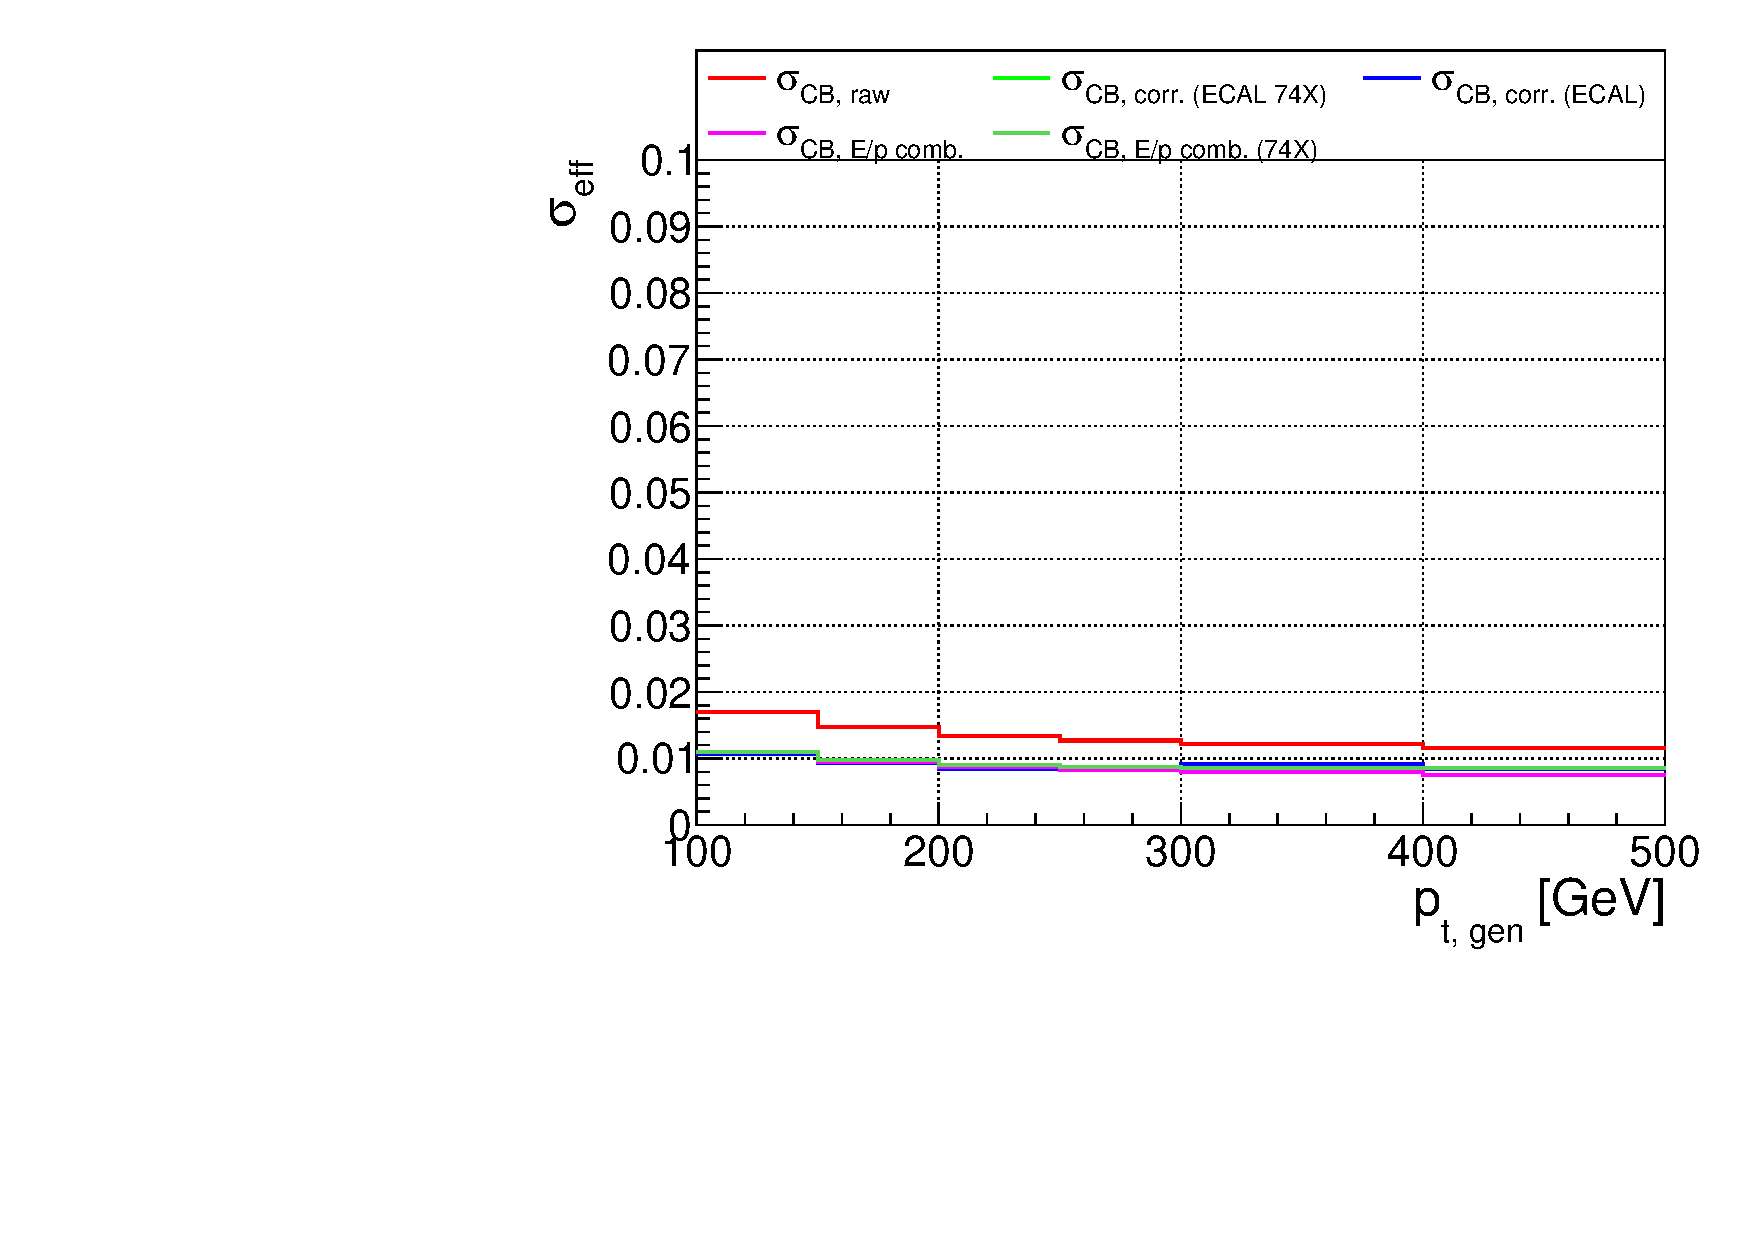
\includegraphics[width=\halflinewidth]{img/regression/pt500_effsigma_electrons.pdf}
    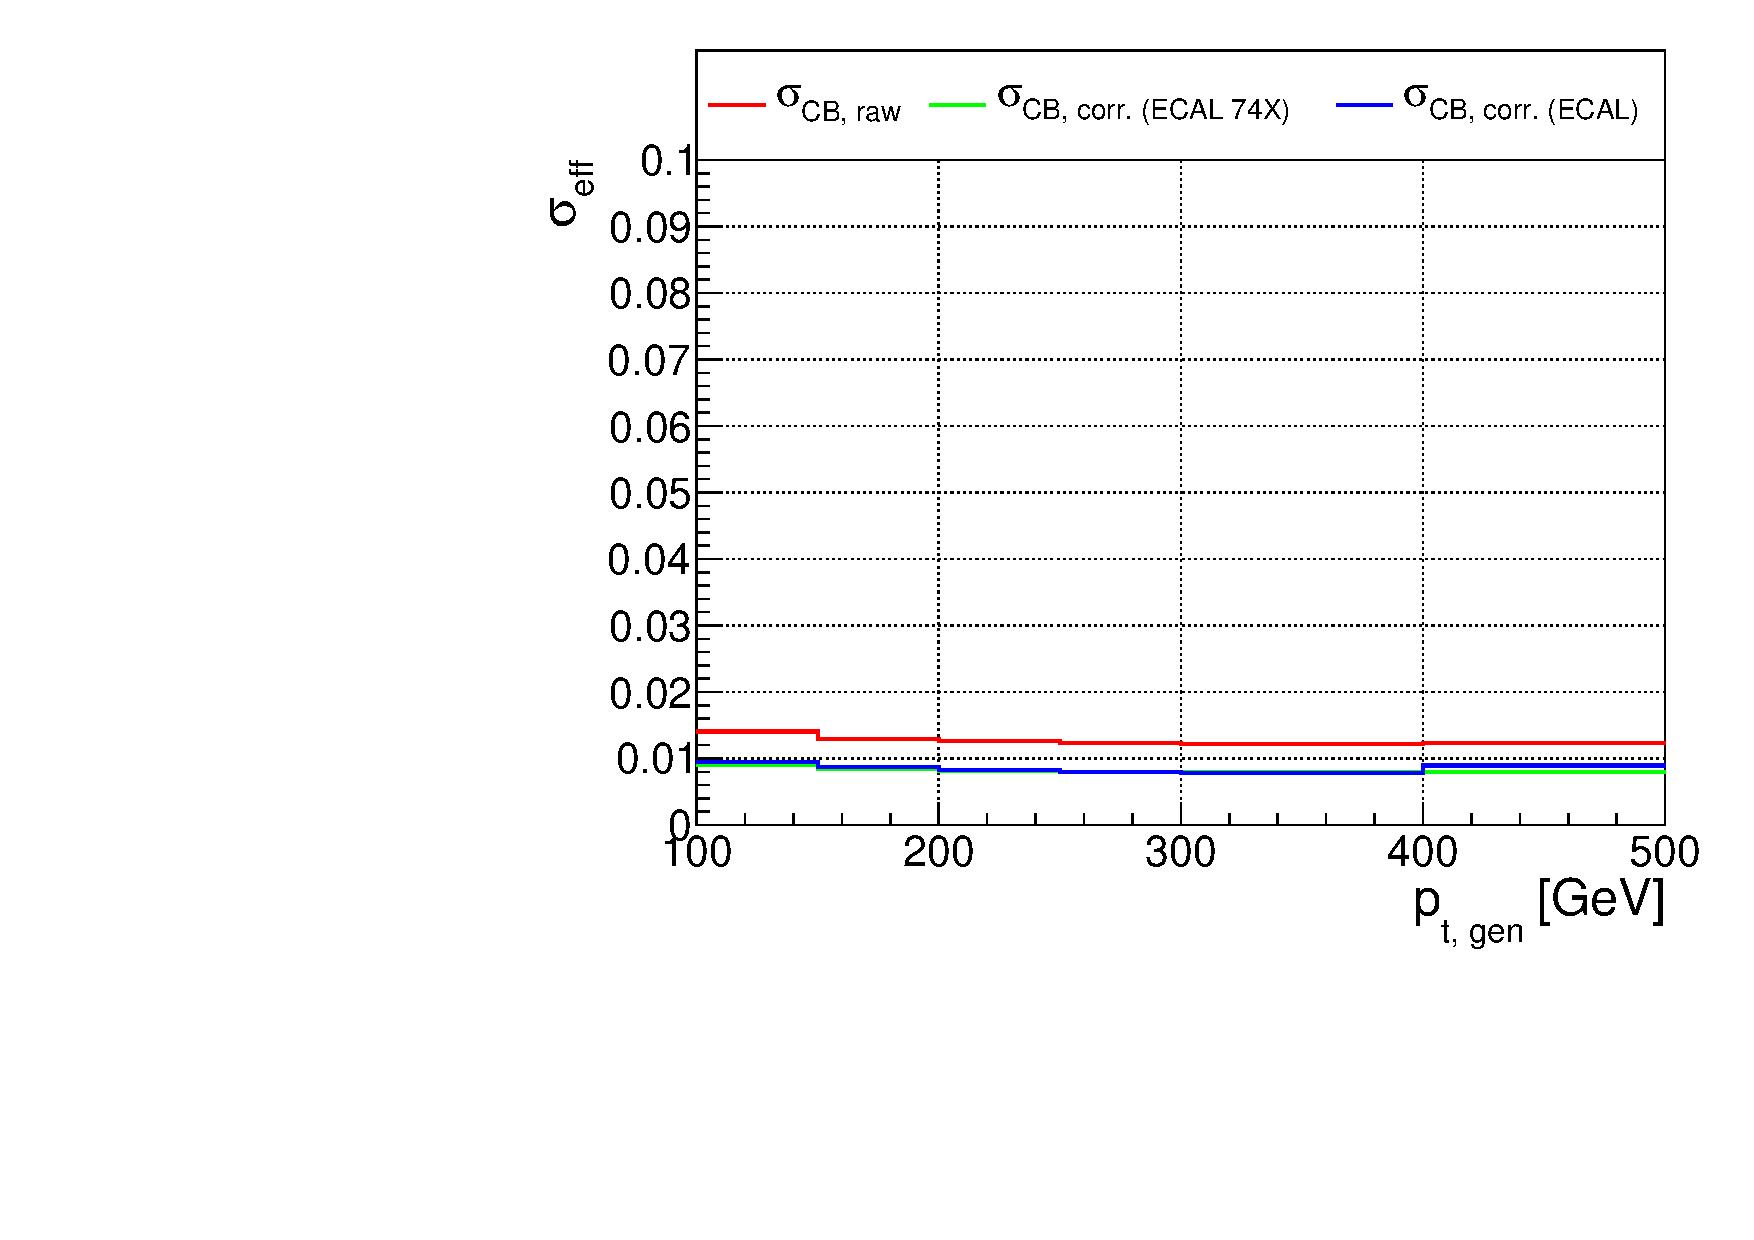
\includegraphics[width=\halflinewidth]{img/regression/pt500_effsigma_photons.pdf}
    \\
    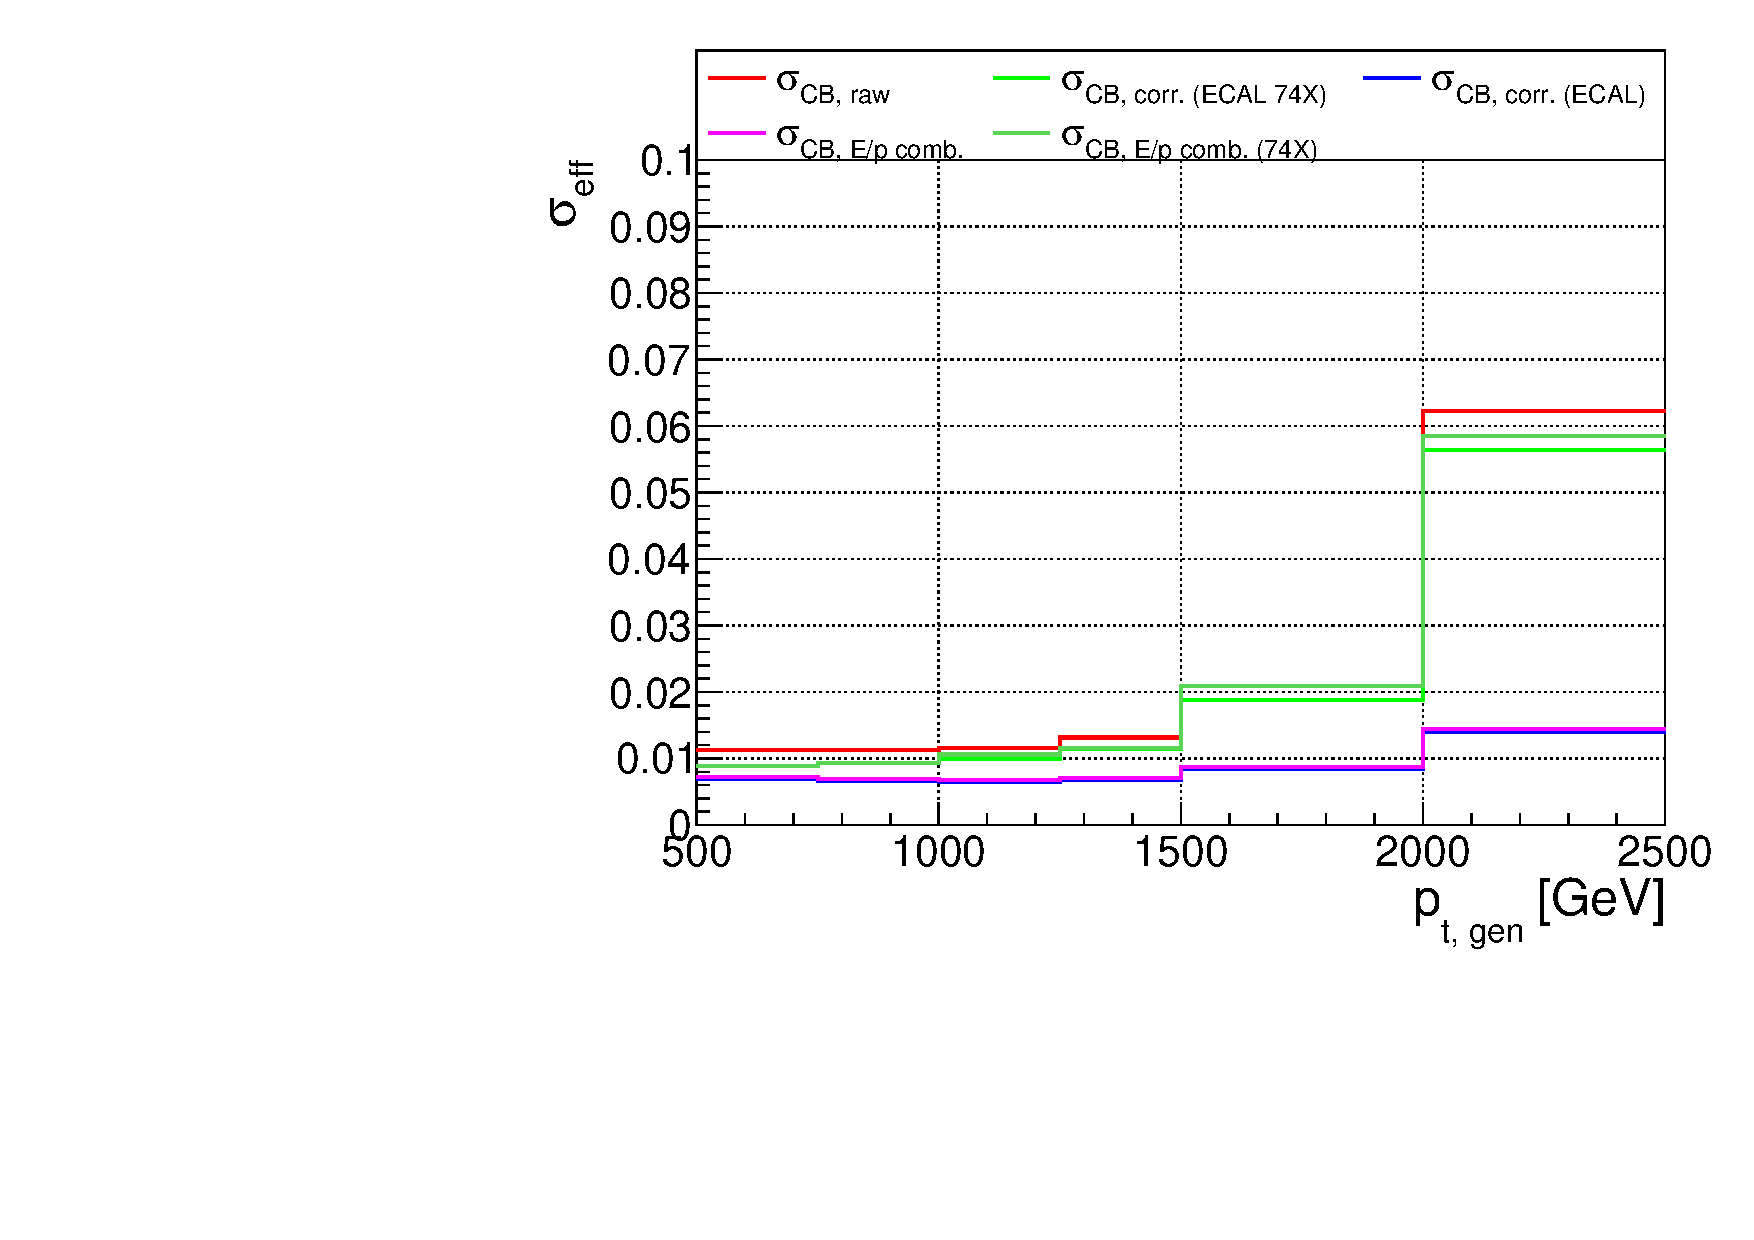
\includegraphics[width=\halflinewidth]{img/regression/pt2500_effsigma_electrons.pdf}
    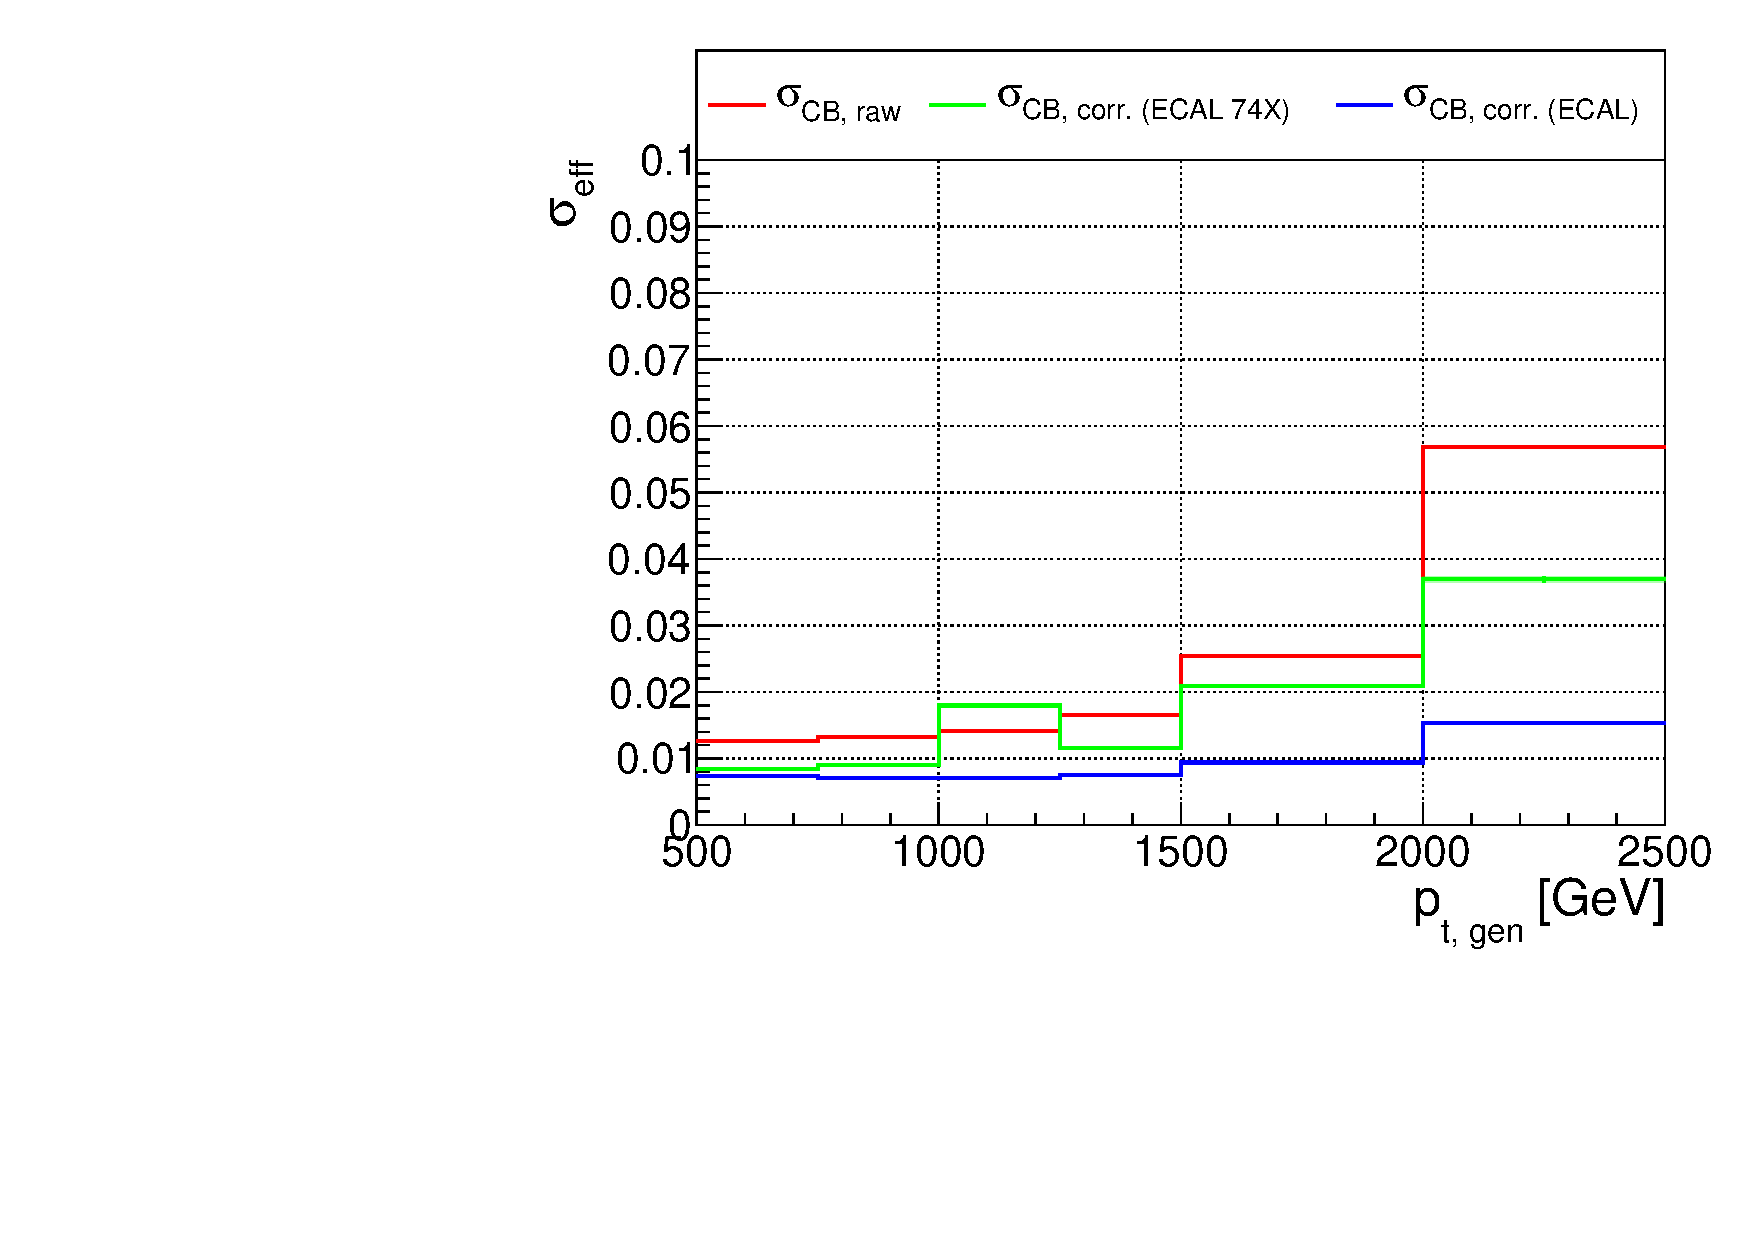
\includegraphics[width=\halflinewidth]{img/regression/pt2500_effsigma_photons.pdf}
    % 
    \caption{
        As in Fig.~\ref{fig:pt100_scale}, but now showing $\sigma_\text{eff}$ instead of the scale, for electrons (left) and photons (right), for various ranges of $\pt$:
        $0 < \pt < 100\GeV$ (top row),
        $100 < \pt < 500\GeV$ (middle row),
        and $500 < \pt < 2500\GeV$ (bottom row).
        }
    \label{fig:effsigma}
  \end{center}
\end{figure}


\begin{figure}[hbtp]
  \begin{center}
    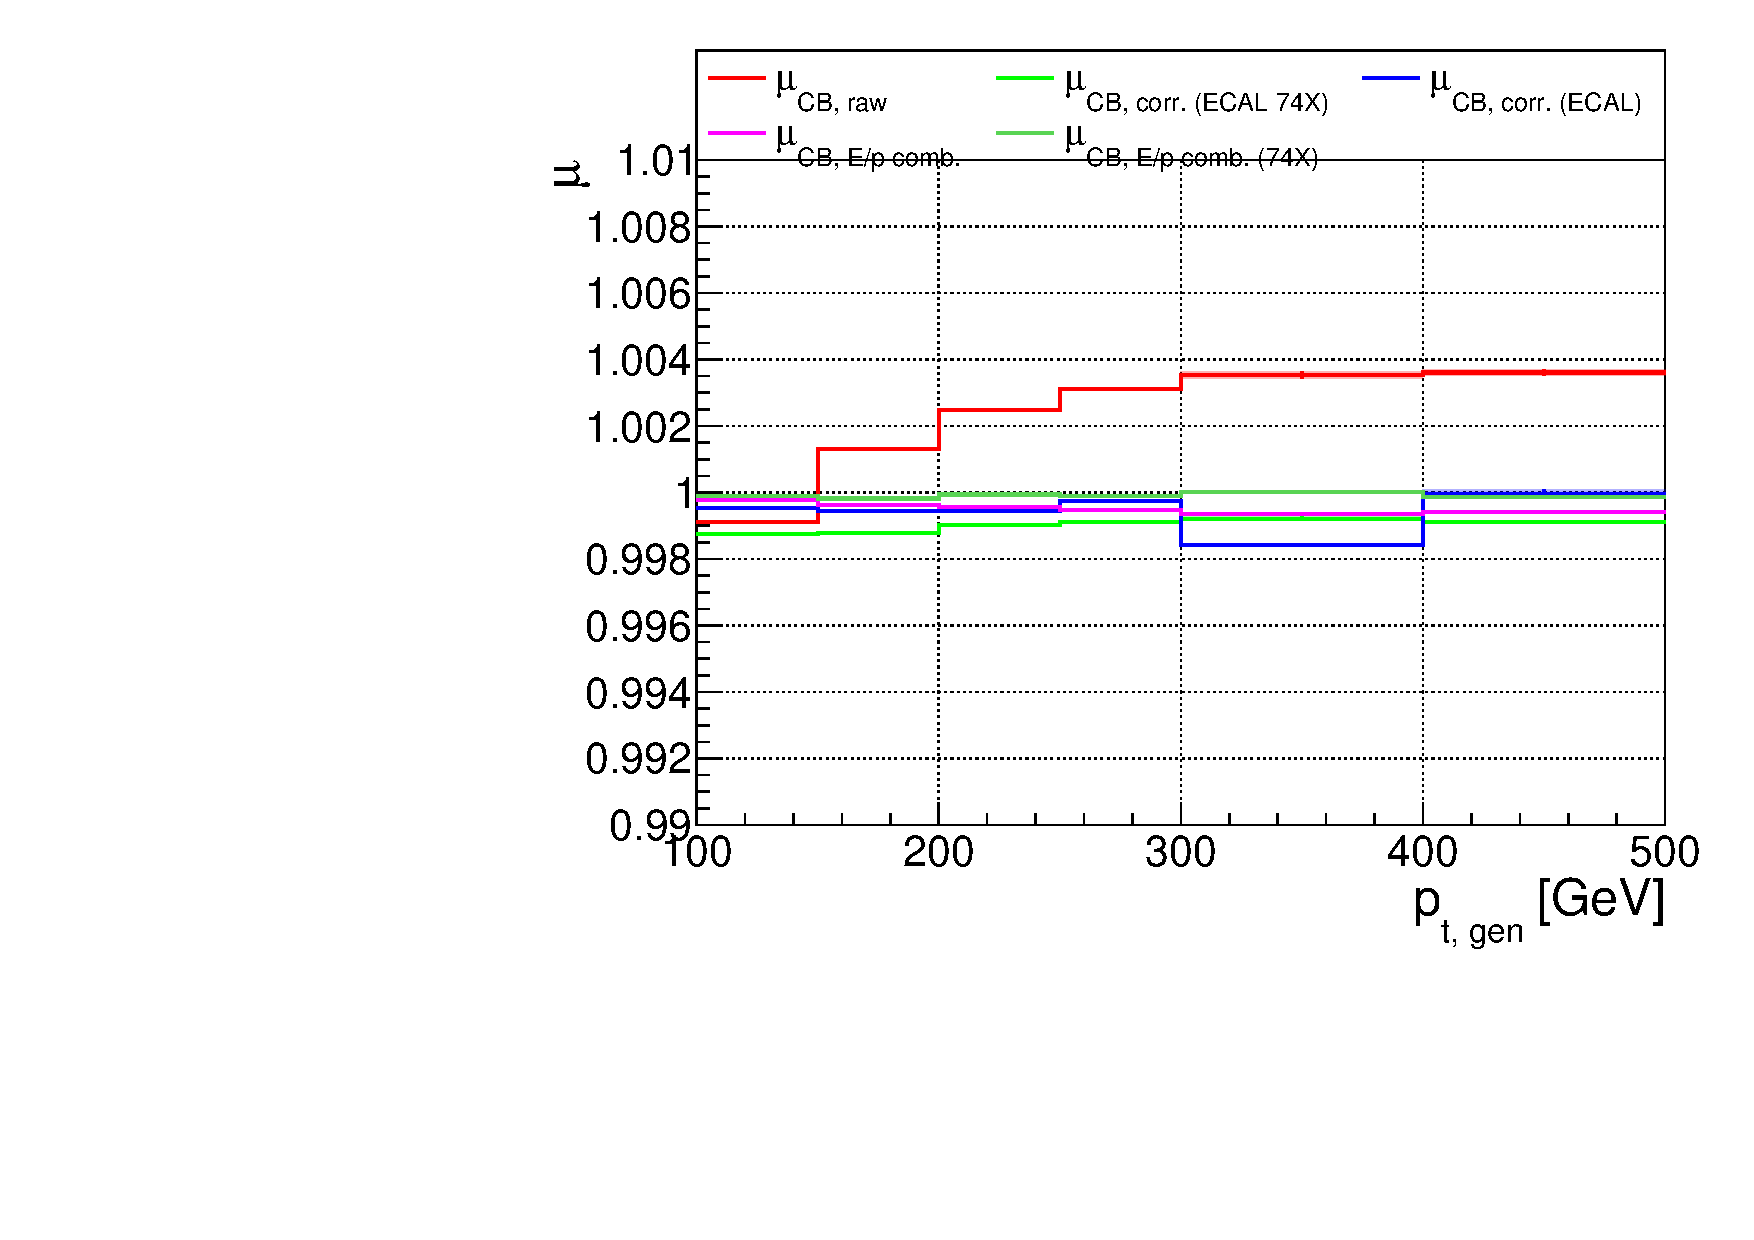
\includegraphics[width=\halflinewidth]{img/regression/pt500_scale_electrons.pdf}
    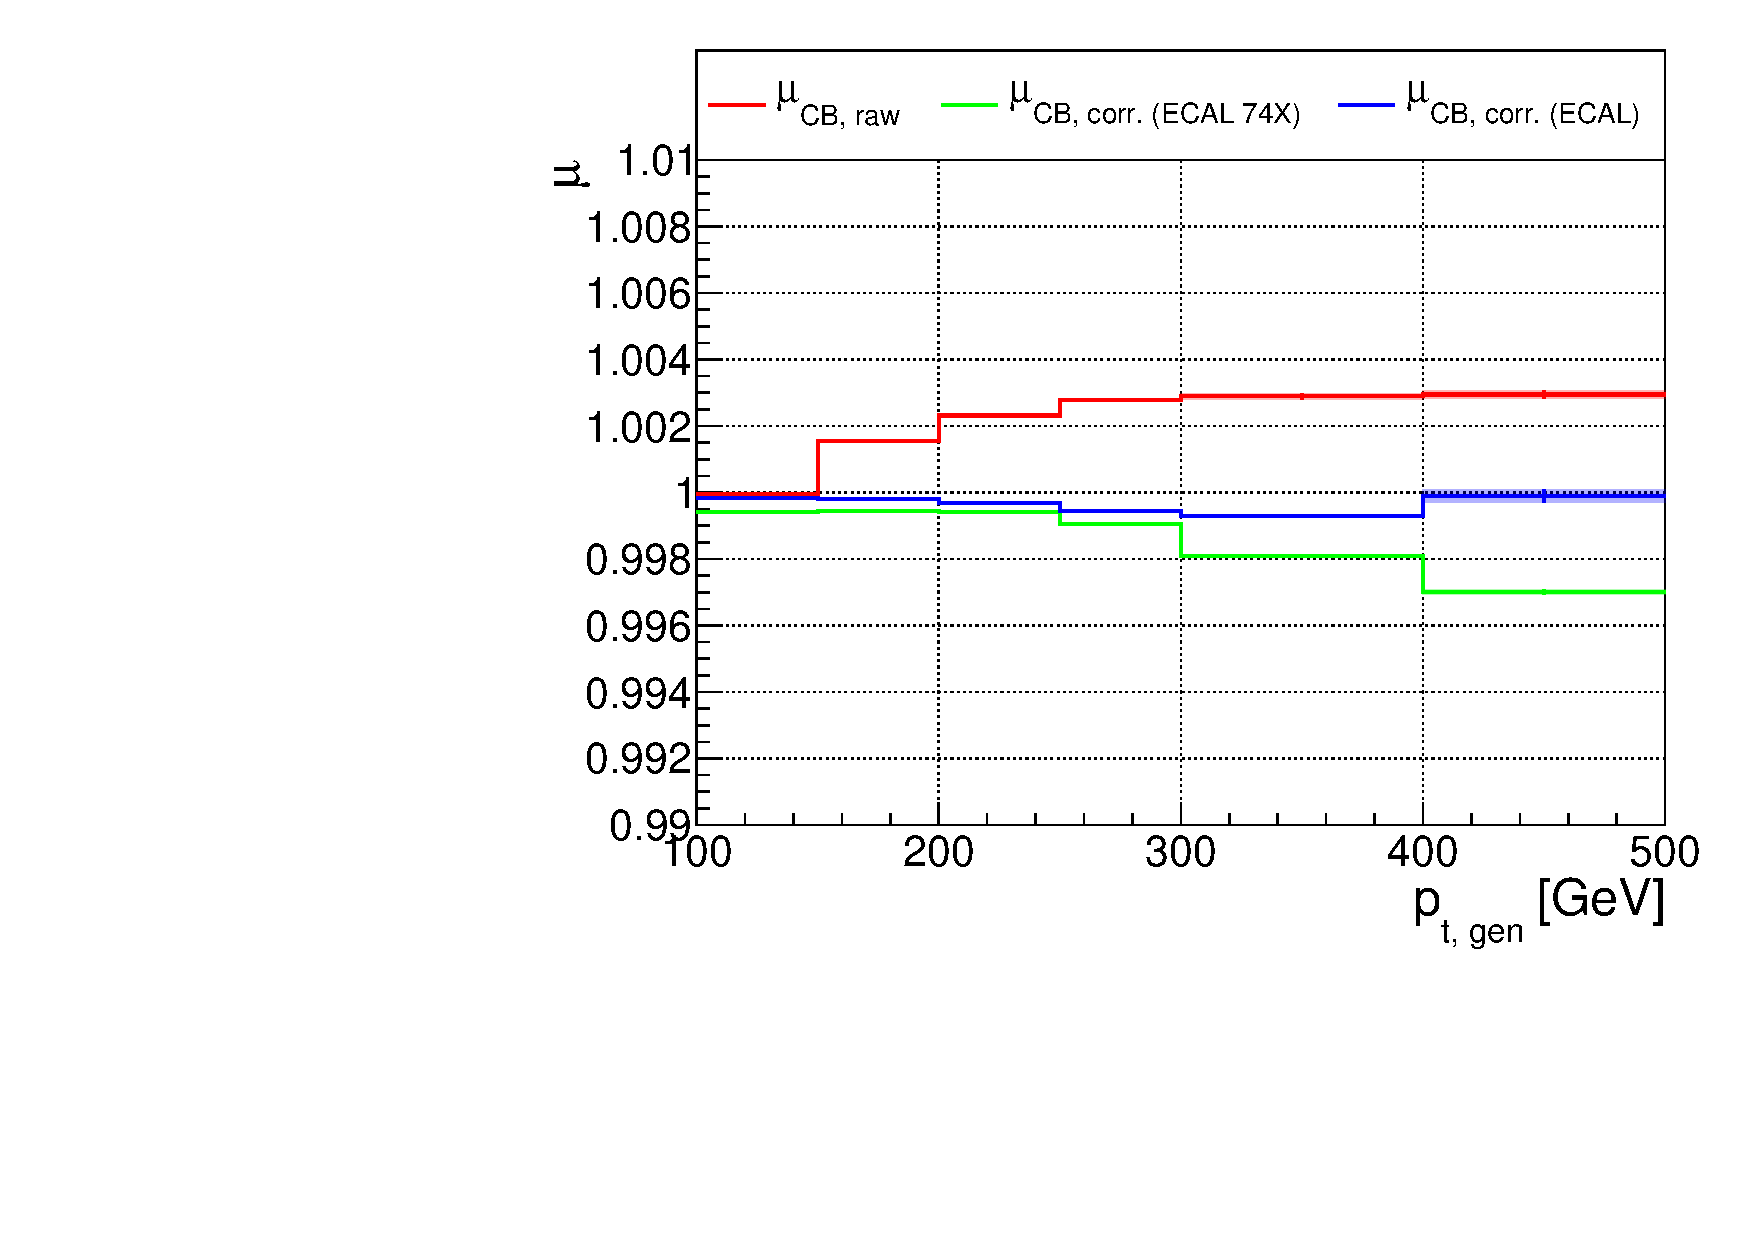
\includegraphics[width=\halflinewidth]{img/regression/pt500_scale_photons.pdf}
    \\
    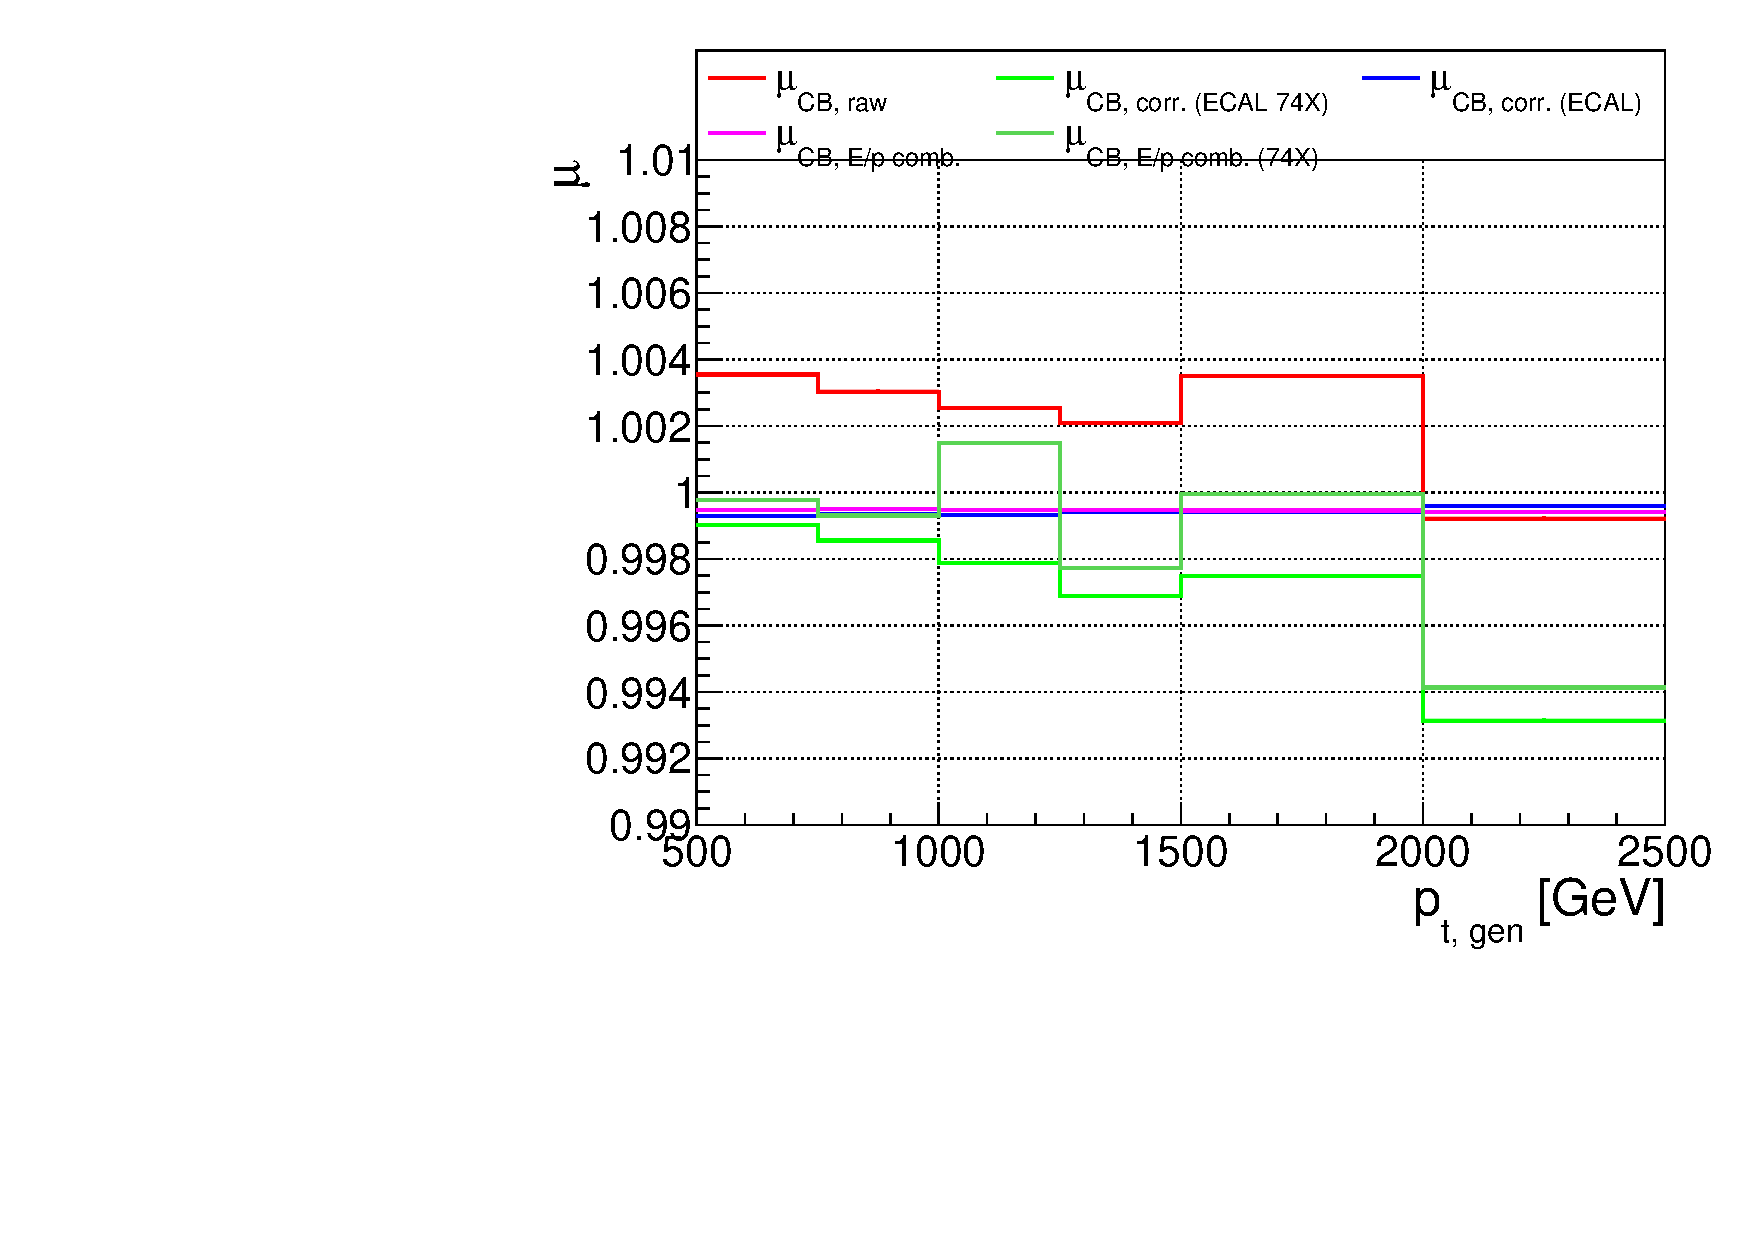
\includegraphics[width=\halflinewidth]{img/regression/pt2500_scale_electrons.pdf}
    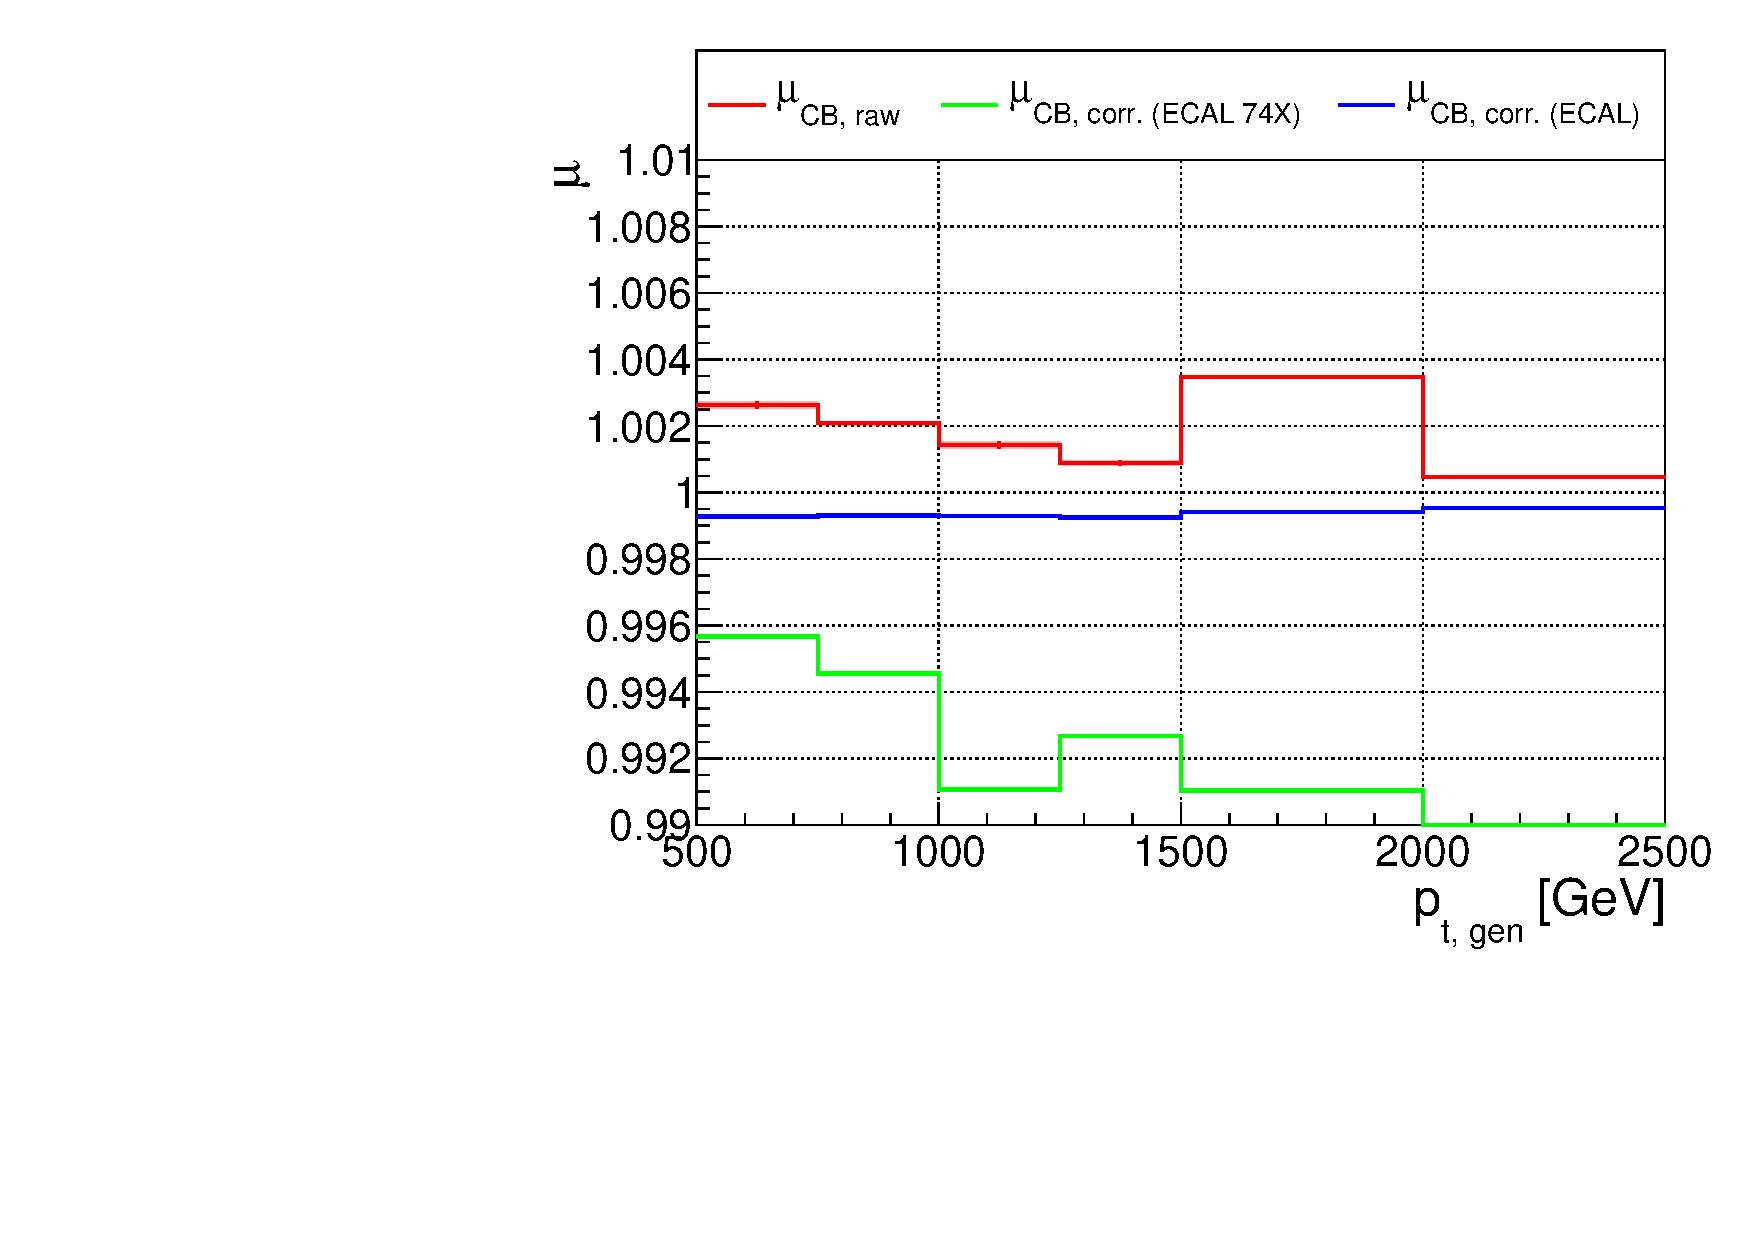
\includegraphics[width=\halflinewidth]{img/regression/pt2500_scale_photons.pdf}
    % 
    \caption{
        As in Fig.~\ref{fig:pt100_scale}, but now for $100 < \pt < 500\GeV$ (top row) and $500 < \pt < 2500\GeV$ (bottom row), for electrons (left) and photons (right).
        }
    \label{fig:pt2500_scale}
  \end{center}
\end{figure}


In summary, the electron and photon energy regression for the 2016 dataset is produced using a two-stage semiparametric BDT in the case of electrons and a single semiparametric BDT in the case of photons.
% 
The new target and training strategy for the electrons significantly improves the quality of the scale in the lower energy regions with respect to previous regressions.
% 
The inclusion of information pertaining to crystal saturation in the training drastically improves the performance of the regression at higher energies; for this region of phase space, the new energy regression is the only reliable energy estimate.


